\chapter{Evaluation}
\label{chap:evaluation}
In this chapter, we evaluate two things: how the parameters we have chosen affect our clustering protocol with different network topologies, and how our clustering compares with the original of the \atwo{} protocol. We begin by describing our evaluation setup, which metrics we look at and how we conduct our tests. Next, we describe our evaluation of the clustering parameters for the clustering algorithm. Finally, we present and discuss our evaluation of clustering implemented on \atwo{} and compare it to the original implementation of \atwo{}. We end this chapter with a discussion on the effectiveness of our clustering implementation.

\section{Test Setup}
To test our clustering implementation, we run an unmodified version of the \atwo{} protocol and compare it to our clustering implementation. In this section, we describe our test setup, which topologies we test on, and which metrics we use to measure our results. 


\subsection{Test Environments}
We evaluate our clustering implementation in two different ways, on the Cooja simulator \cite{Osterlind2006-cooja-introduction} and the Flocklab testbed \cite{Lim2013-flocklab-introduction}. Cooja is the default simulator for ContikiOS \cite{Dunkels2004-contiki-introduction}, the operating system that the Chaos and \atwo{} protocols are implemented on \cite{chaos-introduction-paper, a2-introduction-paper}.

\subsection{Topology Details}
\label{subsec:evaluation-topology-details}
In Cooja we create network topologies with 50 nodes randomly placed in different areas, creating different node densities. We start with 50 nodes in a 100x100 meter area and increase the area in steps of 300 meters all the way to 2500x2500 meters. All network topologies are fixed, they do not change between tests. In all tests, we simulate each network for 30 minutes, which gives us approximately 600 rounds of data. We run our tests using 50 nodes for two reasons. First, 50 nodes are enough to see that the clustering service creates several clusters. Second, running these simulations takes a significant amount of time, and it does not scale well when increasing the number of nodes. Currently, simulating 30 minutes with these 50 node topologies takes between 3-6 hours. Moreover, we chose the different areas of deployment from the fact that in Cooja, a network with area 100x100 meters ensures a 1-hop network and at 2500x2500 meters the network is sparse enough for clustering to be disadvantageous.

The Flocklab testbed consists of 27 nodes deployed both indoors and outdoors at ETH Zurich University. Flocklab provides several services such as \textit{general purpose input output} (GPIO) pin tracing, power profiling, and adjustable supply voltage \cite{Lim2013-flocklab-introduction} to make it easy to measure and evaluate the code that is running on the nodes. Our tests log data to the serial output port of an observer node, Flocklab aggregates the data and sends it to us at the end of each test.


\subsection{Metrics}
We consider the following metrics when evaluating clustering on \atwo{}.

\begin{itemize}
    \item \textit{Latency:} The number of slots it takes for the nodes to complete the current application and power down.
    \item \textit{Energy usage:} An estimation of the energy every node uses per round.
    \item \textit{Reliability:} The percentage of rounds all nodes successfully run the application to completion.
\end{itemize}

We measure latency as the number of slots it takes before all nodes have completed the application that is currently running, and power down. Using absolute time would give us the ability to compare our results with other protocols, however, since we are only interested in comparing with \atwo{}, slots is a straightforward metric to use.

We measure the energy consumption of every node using the built-in energy estimation module Energest in Contiki. The energy measurement includes the total energy consumed by the CPU and radio. We then calculate the average energy consumed over all nodes per Energest time unit, which is approximately 1/128 of a second. Only estimating energy usage in software is a limitation to our testing, but it is adequate for making comparisons.

We measure reliability as the number of rounds all nodes receive the correct final value divided by the total number of rounds the max protocol is supposed to be running; that is, we remove the rounds which the nodes spend running the clustering, demote, and join services. During cluster rounds, we count the round as a success if all nodes in every cluster have learned their local maximum. During CH rounds we count the round as a success if all CHs have learned the maximum global value.

There are primarily two reasons we chose these metrics. First, they give a somewhat complete picture of the performance of the protocol. A protocol that is reliable, energy efficient, and fast is probably useful. Second, Landsiedel et al.~and Al Nahas et al.~use comparable metrics when they evaluated the original implementation of Chaos and \atwo{} \cite{chaos-introduction-paper, a2-introduction-paper}, using comparable metrics will allow for more straightforward comparison. 

\subsection{Limitations}
We limit our evaluation in the following ways. We only compare our clustering implementation to the \atwo{} protocol. Furthermore, we limit the testing to Cooja simulations and tests run on the Flocklab testbed. The simulations will not represent reality in its entirety, as is the case with all simulations. However, we believe that it will still provide valuable results. In contrast, the Flocklab testbed is a WSN with real nodes, but the size of the network limits us. The Flocklab testbed contains 27 nodes, which could be a too small amount to notice any significant performance improvements due to clustering.

Furthermore, we only simulate networks with 50 nodes when testing the parameters, when comparing clustering to the original \atwo{} protocol we also simulate networks with 200 nodes. We choose these node counts since 50 nodes are approximately the maximum number of nodes we can simulate in a reasonable amount of time, allowing us to repeat those tests many times. 200 nodes, on the other hand, takes a very long time to simulate, which is why we only simulated these large networks when comparing our work to the  \atwo{} protocol.

Lastly, we only evaluate clustering using the max application. The max application is the most straightforward application currently implemented on top of the \atwo{} protocol. We have not considered any other application, but it should be possible to modify most of the applications to fit our clustering protocol.

\section{Clustering Parameters}
\label{sec:clustering-parameters}
In this section, we experimentally search for optimal values for the parameters of our clustering algorithm. The parameters are \emph{round re-synchronisation threshold}, \emph{competition radius}, \emph{minimum cluster size}, and \emph{nodes per cluster ratio}; the purpose of these parameters is described in \cref{design:configuration-parameters}. We run each test three to six times and calculate the mean and standard deviation of the reliability of each test configuration for each network topology.

We are primarily interested in reliability for these tests since reliability displays the most significant changes. There are no significant differences in the latency for different values of these parameters; we include the latency results in \cref{app:a} for completeness but will not comment on them any further for the parameter tests. We do, however, get back to latency in the comparison to the \atwo{} protocol.

We use a different number of topologies depending on what parameter we evaluate.  When evaluating the parameter competition radius we test on all network topologies we list in \cref{subsec:evaluation-topology-details} since that parameter is very dependent on the density of the network. When we test the parameters minimum node count and nodes per cluster ratio, however, we use a slightly different setup.

For both of those parameters, we only run tests on topologies ranging from 100x100 to 1300x1300 meters in size, using competition radius 1. We argue that increasing the competition radius while simultaneously increasing the area of the networks will not give any new significant results. By excluding the network topologies with a larger area, we could repeat each configuration for these tests a total of six times, instead of three.

Also, to limit the scope of our evaluation, we use the values listed in \cref{tab:parameter-default-values} for the parameters that we are not currently evaluating. We choose these particular values since we consider them to be sensible defaults. Initial tests using these parameter values gave satisfying results. However, to get a better understanding, we could evaluate how the different parameters interact with each other, but we will not perform those evaluations in this thesis.

\begin{table}[bt]
\centering
\caption{The parameters we evaluate and their default values}
\label{tab:parameter-default-values}
\begin{tabular}{r|l}
\textbf{Parameter}                 & \textbf{Value} \\ \hline
Competition Radius                 & 1              \\
Minimum node count                 & 4              \\
Nodes per cluster ratio            & 10             \\
Round re-synchronisation threshold & 3             
\end{tabular}
\end{table}


\begin{figure}[H]
\centering
\begin{subfigure}{\textwidth}
    \centering
    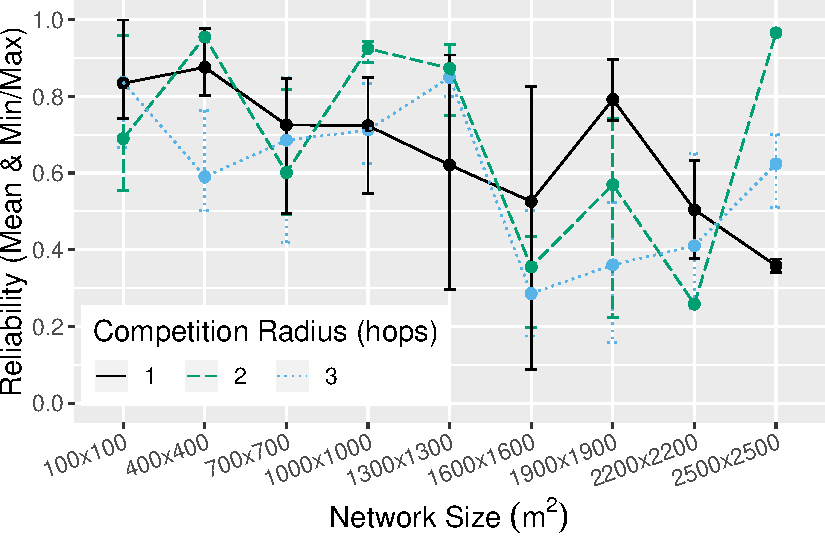
\includegraphics[width=\textwidth, keepaspectratio]{figure/Results/ParameterEvaluation/ResyncThreshold1_Reliability.pdf}
    \caption{Re-synchronisation threshold 1.}
    \label{subfig:resync-treshold-1}
\end{subfigure}
\begin{subfigure}{\textwidth}
    \centering
    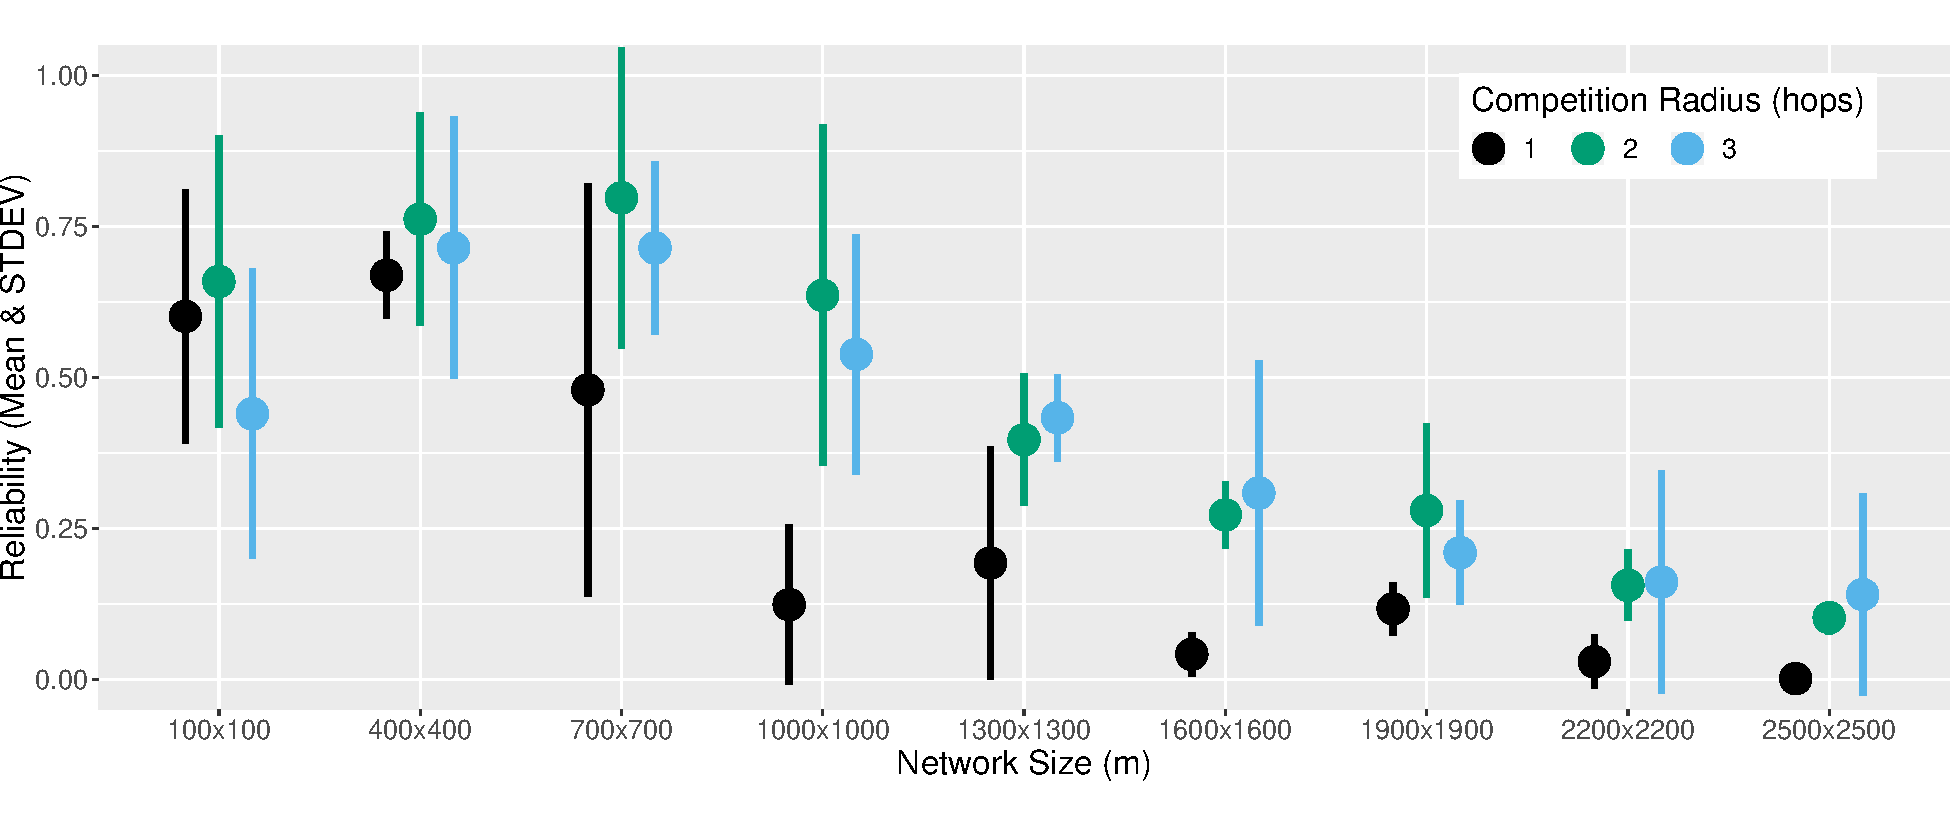
\includegraphics[width=\textwidth, keepaspectratio]{figure/Results/ParameterEvaluation/ResyncThreshold2_Reliability.pdf}
    \caption{Re-synchronisation threshold 2.}
    \label{subfig:resync-treshold-2}
\end{subfigure}
\begin{subfigure}{\textwidth}
    \centering
    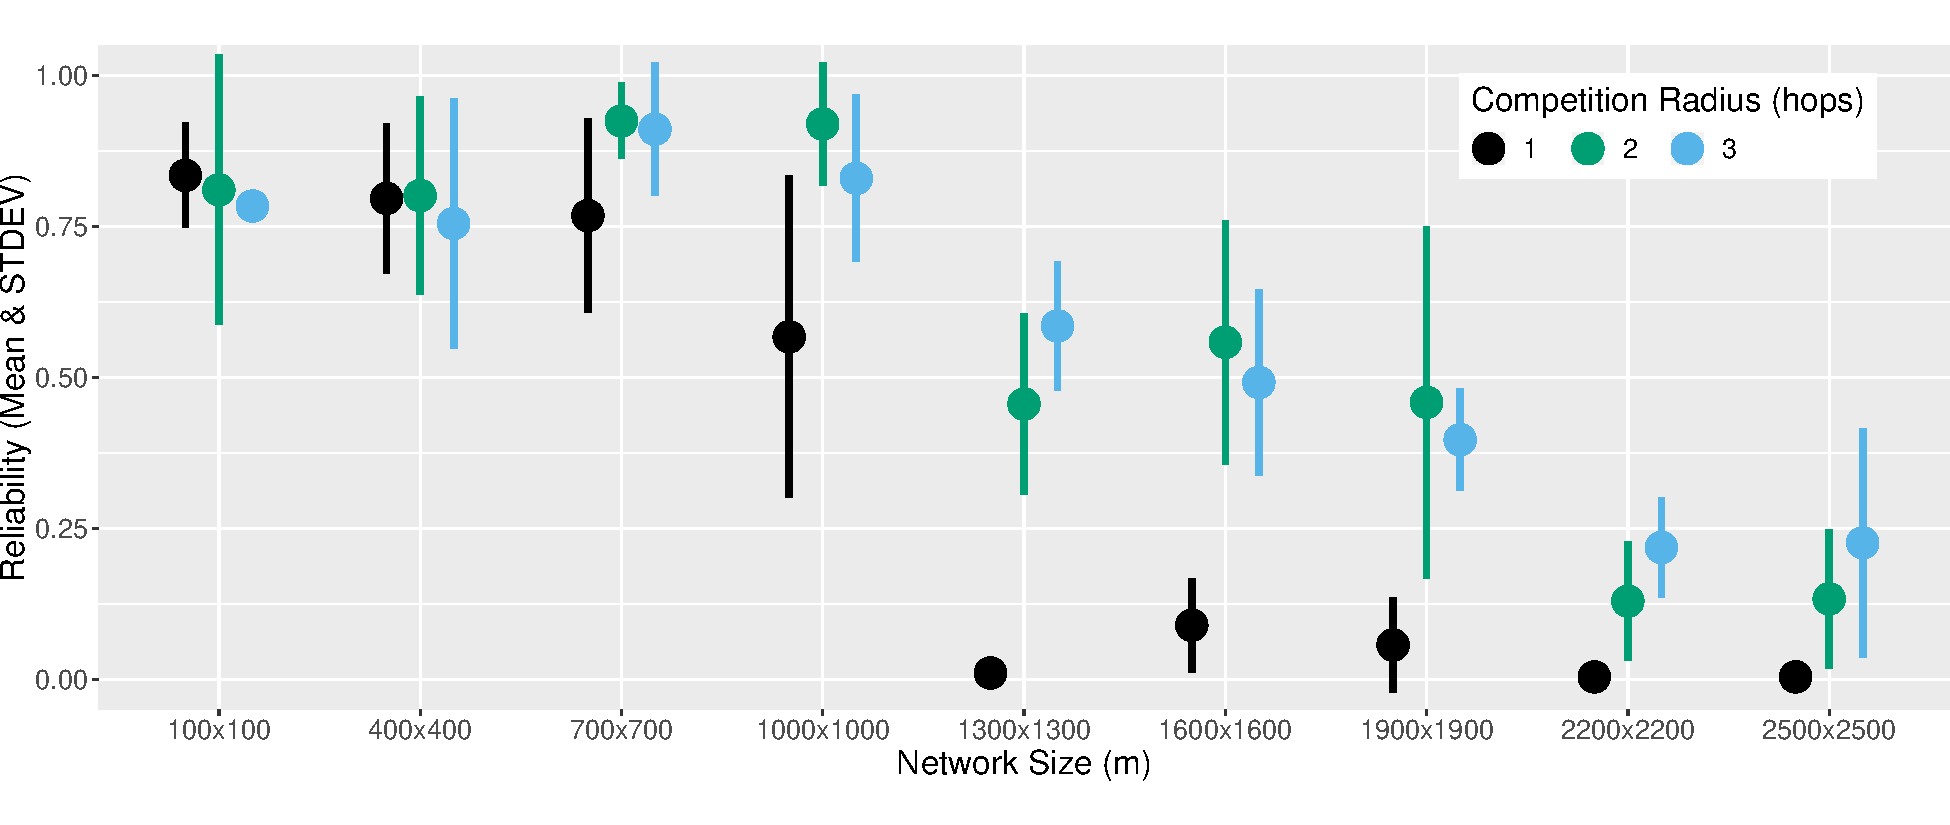
\includegraphics[width=\textwidth, keepaspectratio]{figure/Results/ParameterEvaluation/ResyncThreshold3_Reliability.pdf}
    \caption{Re-synchronisation threshold 3.}
    \label{subfig:resync-treshold-3}
\end{subfigure}

    \caption{Competition radii tests for different values of resynchronisation threshold. The reliability increases as the re-sync threshold increases.}
    \label{fig:resync-treshold-tests}
\end{figure}

\subsection{Round Re-synchronisation Threshold}
The \emph{round re-sync threshold} parameter is not directly related to the clustering algorithm. Instead, it is a setting that controls a fundamental part of the original \atwo{} protocol. Round re-sync threshold is a numeric parameter that determines how many rounds a node can execute without receiving any packet before trying to associate with the network again. 

We briefly evaluate different values for round re-sync threshold since initial testing showed that our clustering implementation is unstable. We started our tests using a re-sync threshold of 1 but that proved to be too strict, and we did not get satisfying results. We evaluate three different values of the round re-sync threshold (1, 2, and 3), for each value of re-sync threshold we evaluate three different values of competition radius (1, 2, and 3), which gives us a total of 9 test configurations.

Looking at the results, we see an increase in stability when we increase the re-sync threshold. The reason for this dramatic increase is due to two things. First, our clustering implementations instability is due to specific scenarios occurring, such as when switching between initiators, which we describe in \cref{subsec:implementation_the-initiator}. Second, when clustering a network, each node generally has fewer chances to successfully receive a packet from another node since it will only listen to nodes from its cluster. This is apparent in our testing setup since we use a relatively small number of nodes and we run many tests on sparser networks, specifically 1300x1300 meters and upwards. 

From this evaluation, we conclude that using a re-sync threshold of 3 is currently the best value for our clustering implementation. We did not test larger values of this parameter due to time constraints. All further evaluation of our clustering implementation uses a re-synchronisation threshold of 3.

\begin{figure}[bt]
    \centering
    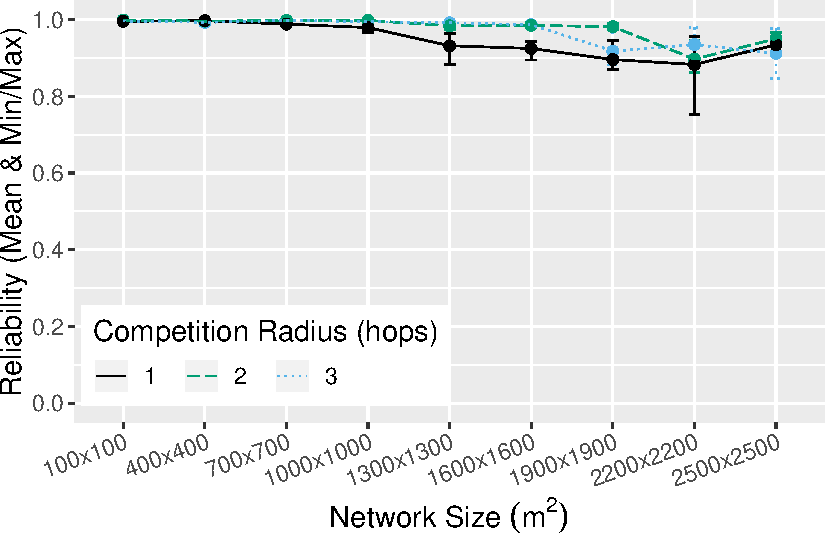
\includegraphics[width=\textwidth, keepaspectratio]{figure/Results/ParameterEvaluation/CompetitionRadius_Reliability.pdf}
    \caption{The reliability for different network sizes. Each network size has been tested with competition radius 1, 2, and 3 (from left to right).}
    \label{fig:comp-radius-reliability}
\end{figure}

\subsection{Competition Radius}
Competition radius is a distance metric measured in hops. A node chooses a CH from all CHs that are closer than the value of the competition radius. We evaluate competition radius with the setup described in \cref{subsec:evaluation-topology-details} with competition radii 1,2 and 3. When looking at the different competition radii, we are mainly interested in how the reliability varies when the density of the network decreases. We show the average reliability and the standard deviation for each network setup and each competition radius in \cref{fig:comp-radius-reliability}. We see some expected results, for networks that are not very dense (e.g. network sizes from 1300x1300 to 2500x2500 meters) using a competition radius of 1 results in worse reliability than for competition radius 2 or 3. We probably get lower reliability for lower density networks because our clustering algorithm will create too many clusters and make the network even sparser, hindering communication. Even though reliability increases when we use competition radius 2 or 3 in large networks it is not by too much, it is still inefficient to cluster large networks with few nodes. 

Furthermore, we do not see any significant difference in the reliability for dense networks when increasing the competition radius. The reliability does not change because in very dense networks with a one-hop diameter, such as the network with an area of 100x100 meters, the competition radius is effectively always one since there are no nodes more than one hop away from any other node.

\subsection{Minimum Node Count}
CHs use the parameter minimum node count during the demote service to decide if they should demote themselves because their clusters are too small. We evaluate this parameter using three different values 2, 4 and off; when the value is off a CH will never demote itself due to having too few nodes in its cluster. We show the mean reliability and standard deviation of these tests in \cref{fig:min-node-count-reliability}.

Looking at the reliability of the different network topologies we see no clear correlation between minimum node count and the reliability on the same topology. The reliability drops, as expected, the sparser the network is.

There are several potential reasons why we can not see any significant difference between different values for this parameter, which can not be determined by looking at the reliability graph alone. First, the impact of having a mix of small and large clusters in a network could be negligible, compared to having more equally sized clusters. The second reason could be that in the tests we ran, the clustering algorithm did not create clusters that were considered to be too small, then the parameter would not have any effect on the reliability. To further investigate the effects of this parameter we could increase the value of the parameter. However, with only 50 nodes in the network increasing it further than we have already done could result in the clustering algorithm creating too few clusters.



\begin{figure}[bt]
    \centering
    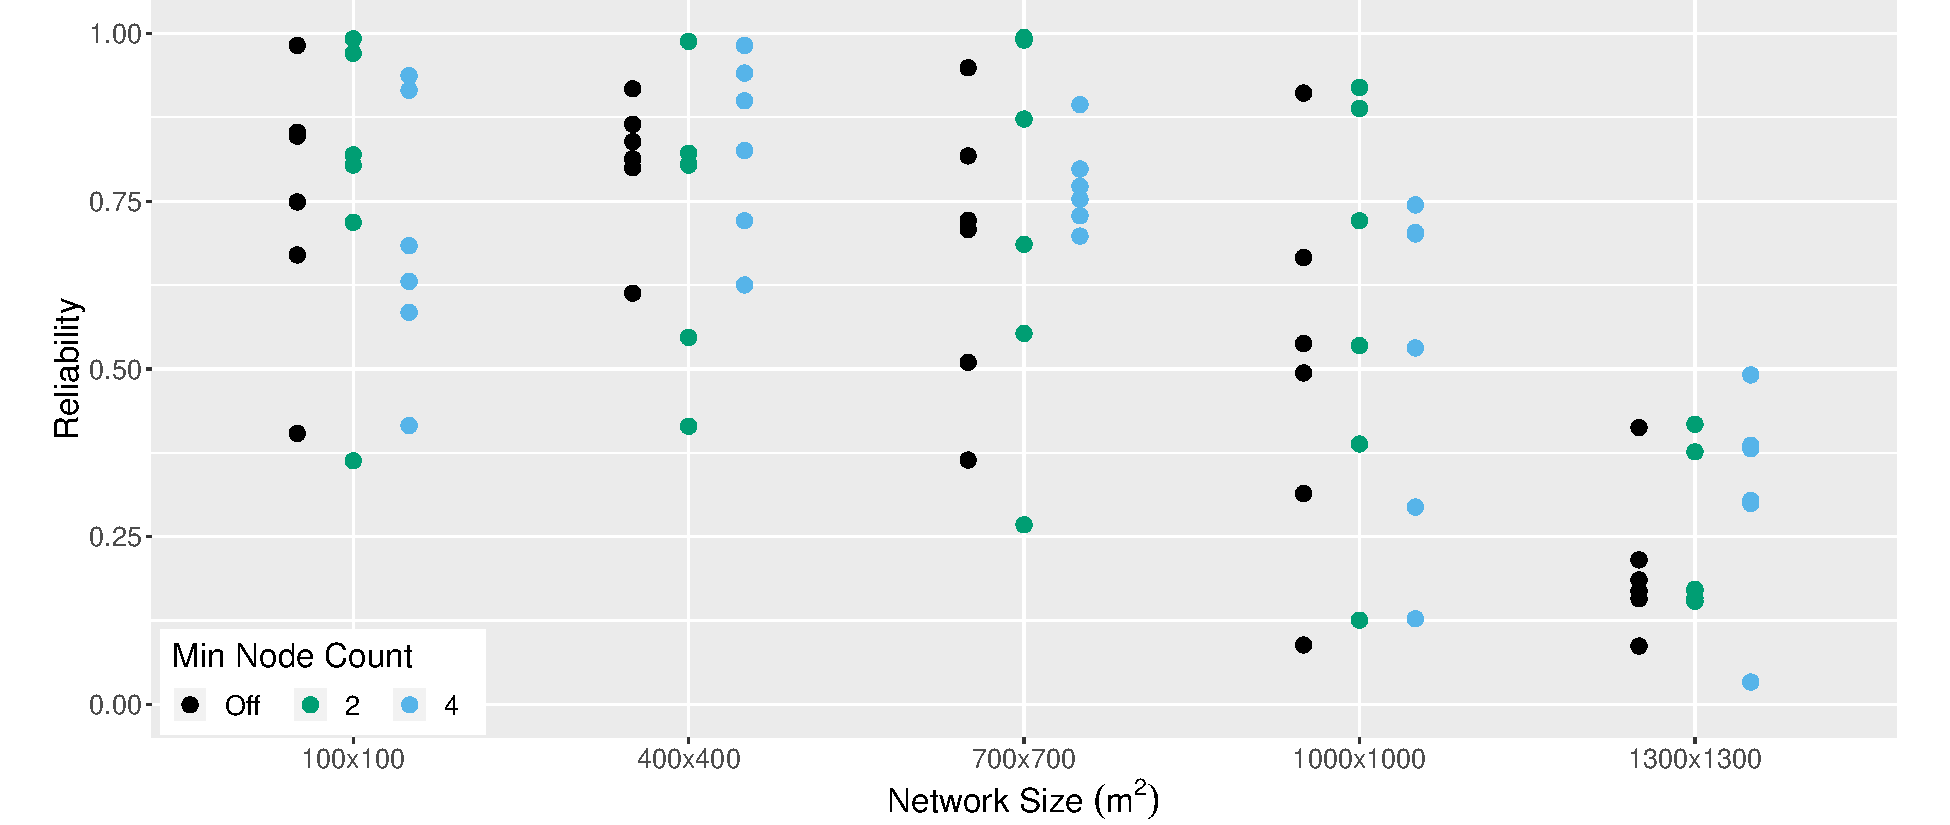
\includegraphics[width=\textwidth, keepaspectratio]{figure/Results/ParameterEvaluation/MinNodeCount_Reliability.pdf}
    \caption{The reliability for different network sizes. Each network has been tested with minimum node count values off, 2, and 4 (from left to right).}
    \label{fig:min-node-count-reliability}
\end{figure}

\subsection{Nodes per Cluster Ratio}
Nodes use the \emph{nodes per cluster ratio} parameter to determine if they may elect themselves even if they have heard another CH within the chosen competition radius. The parameter describes a ratio of how many neighbours needs to be in the vicinity of the node relative to how many CHs it has as neighbours. We test the values 5, 10, 15, and off for this parameter. The value off means a CH may never announce itself if it has heard another CH within the network's competition radius; it is comparable to having an arbitrarily large value for the parameter. The results can be seen in \cref{fig:nodes-per-cluster-ratio-reliability}.


When we looked closer at the results with good reliability, the trend is that the fewer clusters the algorithm created, the better the reliability is. When max node count is turned off, dense networks (100x100) only elect one CH which mostly makes the network run like \atwo{} without clustering, hence the excellent reliability results. Similarly, only one CH is elected in four out of the six tests comprising the data labelled as 400x400 with max node count set to off. The two cases in which more clusters were created are the tests with the lowest reliability, causing a lower mean and a more substantial standard deviation compared to the 100x100 tests. We can also see that when we use a value of 5, the reliability drops significantly since too many clusters are created; in some cases, for these tests, approximately 20 clusters were created. Consequently, as the value of \emph{nodes per cluster ratio} increases, we also see an increase in the mean reliability.



\begin{figure}[bt]
    \centering
    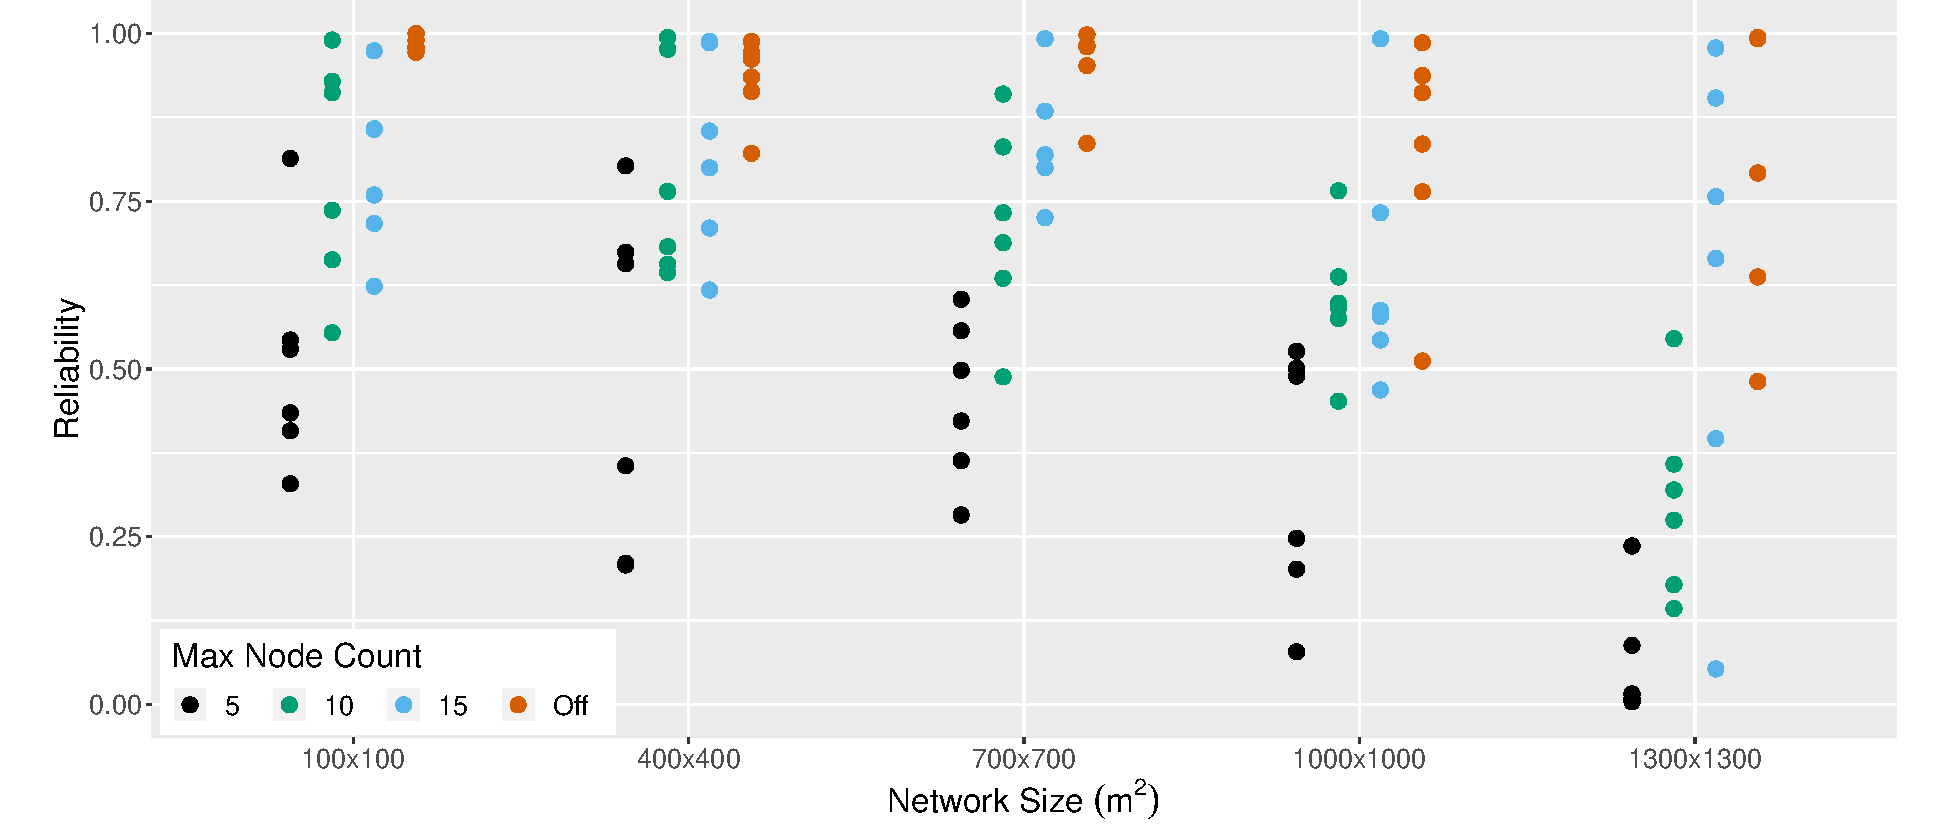
\includegraphics[width=\textwidth, keepaspectratio]{figure/Results/ParameterEvaluation/MaxNodeCount_Reliability.pdf}
    \caption{The reliability for different network sizes. Each network size has been tested with max node count off, 5, 10, and 15 (from left to right).}
    \label{fig:nodes-per-cluster-ratio-reliability}
\end{figure}


\subsection{Discussion}
The results we see in the parameter evaluation vary greatly, both when looking at a single test but also when looking at the different evaluations of the parameters combined. For some parameters, like competition radius, we see a significant increase in reliability as the network area increases for higher values of competition radius. For the parameter minimum node count, on the other hand, we see almost no difference in the reliability when the value of the parameter changes. From these results, we can give some general remarks about each of the parameters.


First, for competition radius, we see that this parameter is useful in creating reliable clusters since this is the parameter that overall had the most significant impact on the reliability of a test when increasing the network area. 

Second, for minimum node count, the results we got from these tests suggest that this parameter does not have an impact on the overall reliability of the tests we ran. However, even if this is true, there is still a bad scenario that can occur which this parameter will solve. The scenario is that a node announces itself as CH, but no other nodes join its cluster. When a CH is alone in its cluster, it will, in the current implementation, only run the join application and never the max application. A CH not running the max application will result in lower reliability since we expect all CHs to receive either the local or global maximum value at the end of each round.

We can see an example of this bad scenario occurring by looking at an individual test from the evaluation of minimum node count. This test, which ran on the 700x700 topology, had a bug causing a CH to form a cluster by itself resulting in the reliability $26\%$. Other tests on the same topology achieved much higher reliability, with the highest being $99.4\%$. There are many possible causes to why there might be such a significant difference between the reliability in the best and worst tests. However, we believe the most critical factor is that the test with the lower reliability had a cluster with a single node in it, for 170 of the rounds it should have been running the max application. We show the clusters created for that particular run in \cref{fig:min-node-count-example}, as we can see the CH with id 12 at the top does not have any other node in its cluster.

\begin{figure}[bt]
    \centering
    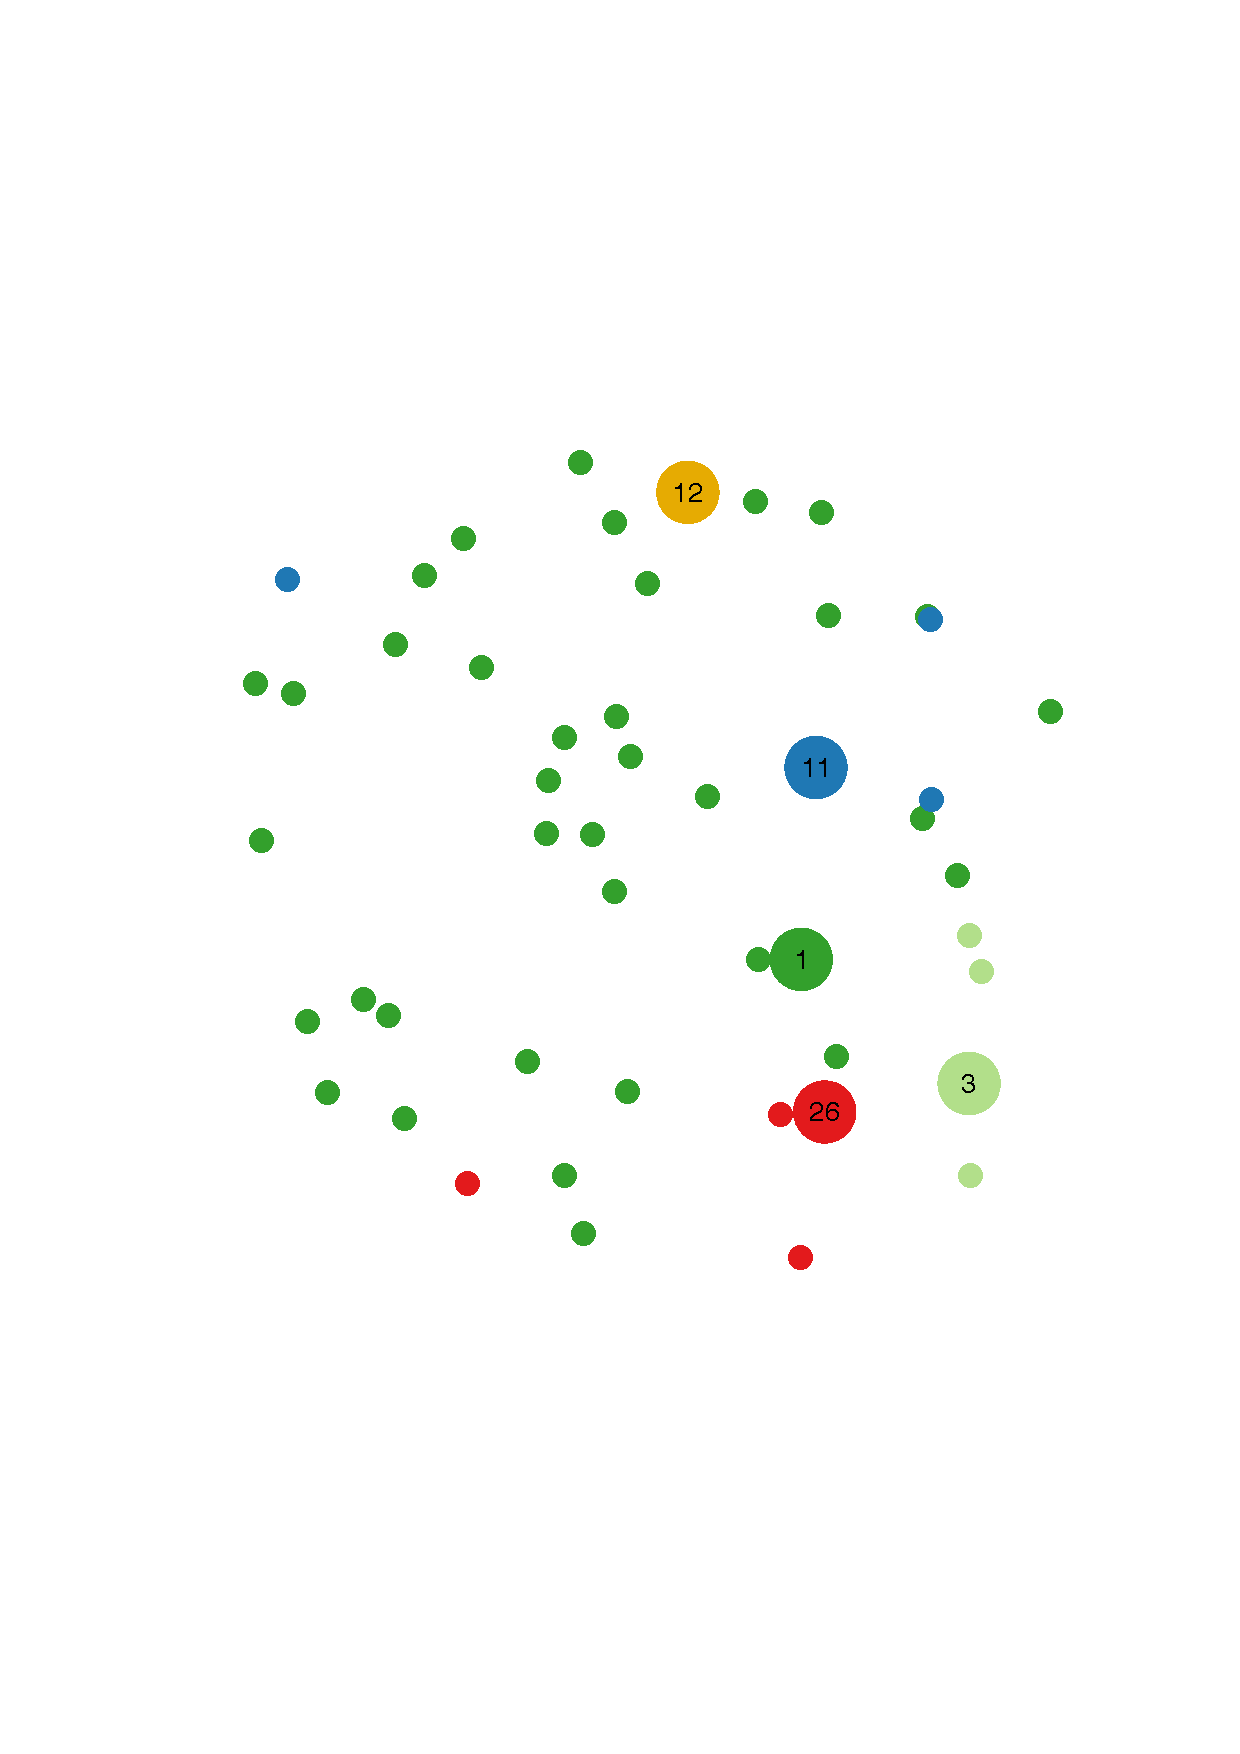
\includegraphics[width=0.5\textwidth]{figure/Results/Discussion/MinNodeCountExample.pdf}
    \caption{An example of a clustering in a 700x700 network which resulted in one CH (node 12) being alone in its cluster. Each colour represents a different cluster, and the larger nodes are CH.}
    \label{fig:min-node-count-example}
\end{figure}

Last, the nodes per cluster ratio parameter worked as we expected. The idea behind this parameter is that since clustering a network should be desirable we want to address the fact that our clustering service is too aggressive when it determined which nodes are allowed to become cluster heads. However, because of the instability in our clustering, the results we got was effectively the opposite, when fewer clusters were created, we got better reliability. Suggesting that this parameter should always be completely turned off.

Nonetheless, we can still consider the parameter useful since it addresses a shortcoming in the algorithm design. For our purpose, the most relevant metric for this parameter is not the reliability of the tests but rather the number of clusters created. We have not performed a rigorous analysis of the results in this regard; however, the data we have looked at suggests that the parameter performs its intended function.



\section{Comparing \atwo{} with Clustering}
In this section, we outline the results we get from evaluating \atwo{} with clustering and compare those results with the results we get from our evaluation of the original \atwo{} protocol. We show results for reliability, latency, and estimated energy usage for all tests we run. We begin by describing the reliability results since they are the most varying and the relevance of the results about latency and energy depend on the reliability of a test.

Note that we have excluded data from two tests (50 nodes in the 2500x2500 topology and 200 nodes in the 400x400 topology) since they suffered the scenario we describe in \cref{subsec:implementation_the-initiator}, i.e., the original initiator starts associating early causing the whole network to get stuck associating. This happened in one out of the three tests we run for each of the two configurations, which means that we calculate the mean and standard deviation from only two data points instead of three. We exclude these tests since they almost never ran the max application, which means that we have no data about the reliability or latency. Furthermore, when the nodes associate they use more energy giving us two outliers in the test results which do not say anything useful about how much energy our clustering protocol consumes.

Furthermore, from our evaluation of the clustering parameters in \cref{sec:clustering-parameters}, we know that different values of some parameters drastically affect the performance of our clustering protocol, especially competition radius. Consequently, we have used different values for some parameters for different network topologies. We change the value of the parameter competition radius as the network size increases for the topologies consisting of 50 nodes, to not create too many clusters in already sparse networks. Additionally, we change the value of the parameter nodes per cluster ratio for the two smallest topologies in the 200 nodes test (100x100 and 400x400), to force the algorithm to create an appropriate amount of clusters in dense networks. We list all topologies we test on and the parameter values that change for the tests in \cref{app:parameter-values-for-the-atwo-comparison}.i


\begin{figure}[bt]
    \centering
    \begin{subfigure}{0.7\textwidth}
        \centering
        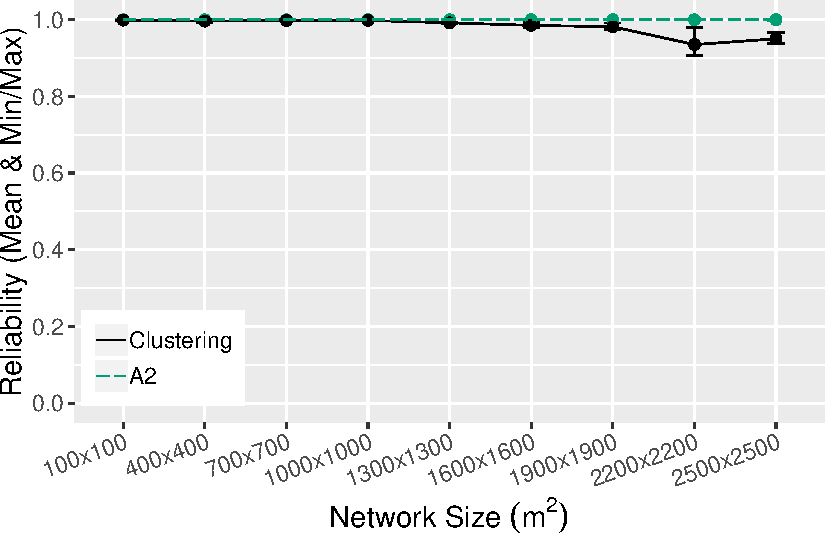
\includegraphics[width=\textwidth]{figure/Results/ChaosComparison/ChaosComparison_50_Reliability.pdf}
        \caption{Networks with 50 nodes.}
        \label{subfig:reliability-50-nodes}
    \end{subfigure}
    \hfill
    \begin{subfigure}{0.7\textwidth}
        \centering
        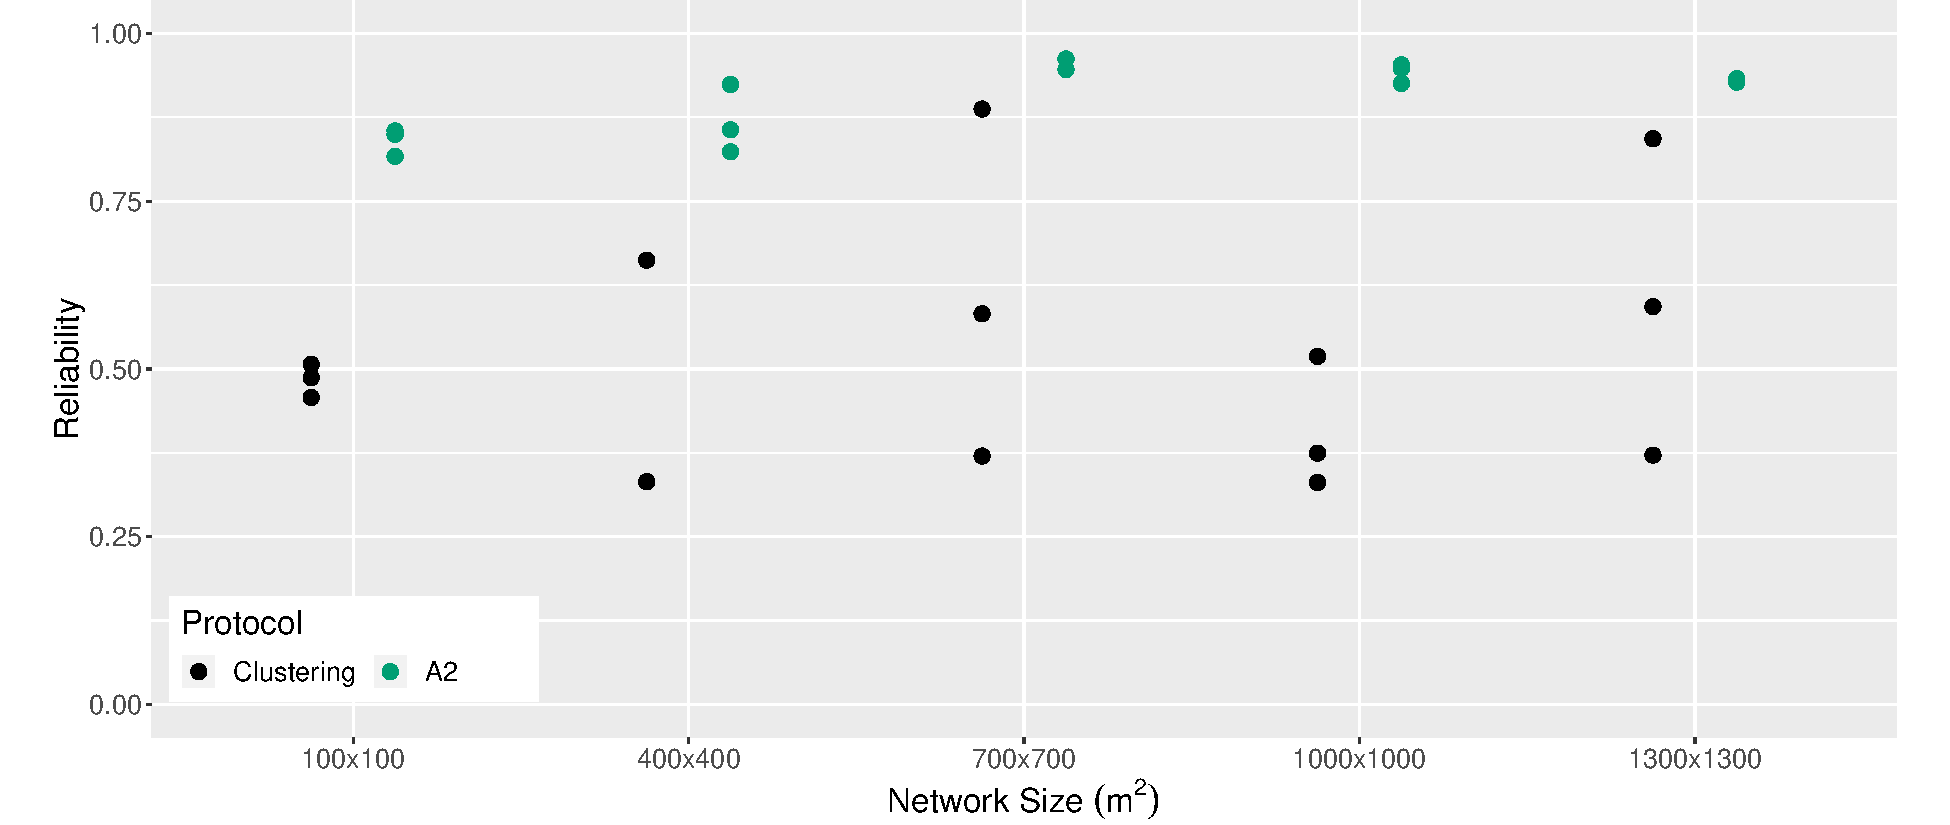
\includegraphics[width=\textwidth]{figure/Results/ChaosComparison/ChaosComparison_200_Reliability.pdf}
        \caption{Networks with 200 nodes.}
        \label{subfig:reliabilty-200-nodes}
    \end{subfigure}
    \caption{Reliability comparison between \atwo{} with clustering and original \atwo{}.}
    \label{fig:reliability-result}
\end{figure}
\subsection{Reliability}
\label{subsec:evaluation-reliability}
As seen in \cref{fig:reliability-result}, \atwo{} outperforms the clustering implementation in reliability in all cases. However, we see some promising results for the clustering implementation in the topology with 50 nodes in an area of 1000x1000 meters, \cref{subfig:reliability-50-nodes}, where two out of three tests has a reliability of more than $97.5$ percent. Both of these tests produced somewhere between two to four clusters in the network. At 1300x1300 meters in \cref{subfig:reliability-50-nodes}, the reliability drops to just below $50\%$ and then continues to decrease as the area of the networks increase. Looking at the results for 50 versus 200 nodes in \cref{subfig:reliability-50-nodes} and \cref{subfig:reliabilty-200-nodes} we compare network topologies from 100x100 up to 1300x1300 meters. When increasing the node count from 50 to 200, the reliability of all tests drop, except for the 1300x1300 topology in the clustering case.


The drop in reliability for \atwo{} is probably due to interference; Al Nahas et al.~\cite{a2-introduction-paper} have already observed and resolved this issue in dense networks by using parallel channels, which we describe in \cref{subsec-frequency-agility}. As we have disabled parallel channels, the reliability is affected. Similarly to parallel channels, clustering should also artificially lower network density and resolve the problem of interference. Hence, we expected a more significant drop in reliability from \atwo{} than in the clustering solution. However, this is not what we observe in the comparison between 50 and 200 nodes. Instead, we see that reliability does not scale to dense networks well with clustering. 

The reliability increase of the 1300x1300 network when moving from 50 to 200 nodes. One cause could be the node density on the 1300x1300 network with 200 nodes is comparable to that of the 700x700 network with 50 nodes. In \cref{subfig:reliability-50-nodes}, we have good results on the 700x700 network with 50 nodes motivating that the node density is suitable for clustering. Further evaluation would include runs of 200 node networks for network sizes bigger than 1300x1300 meters to see if the trend has been shifted. However, it could also be the case that the tests were lucky with the clusters created.

\begin{figure}[bt]
    \centering
    \begin{subfigure}{0.7\textwidth}
        \centering
        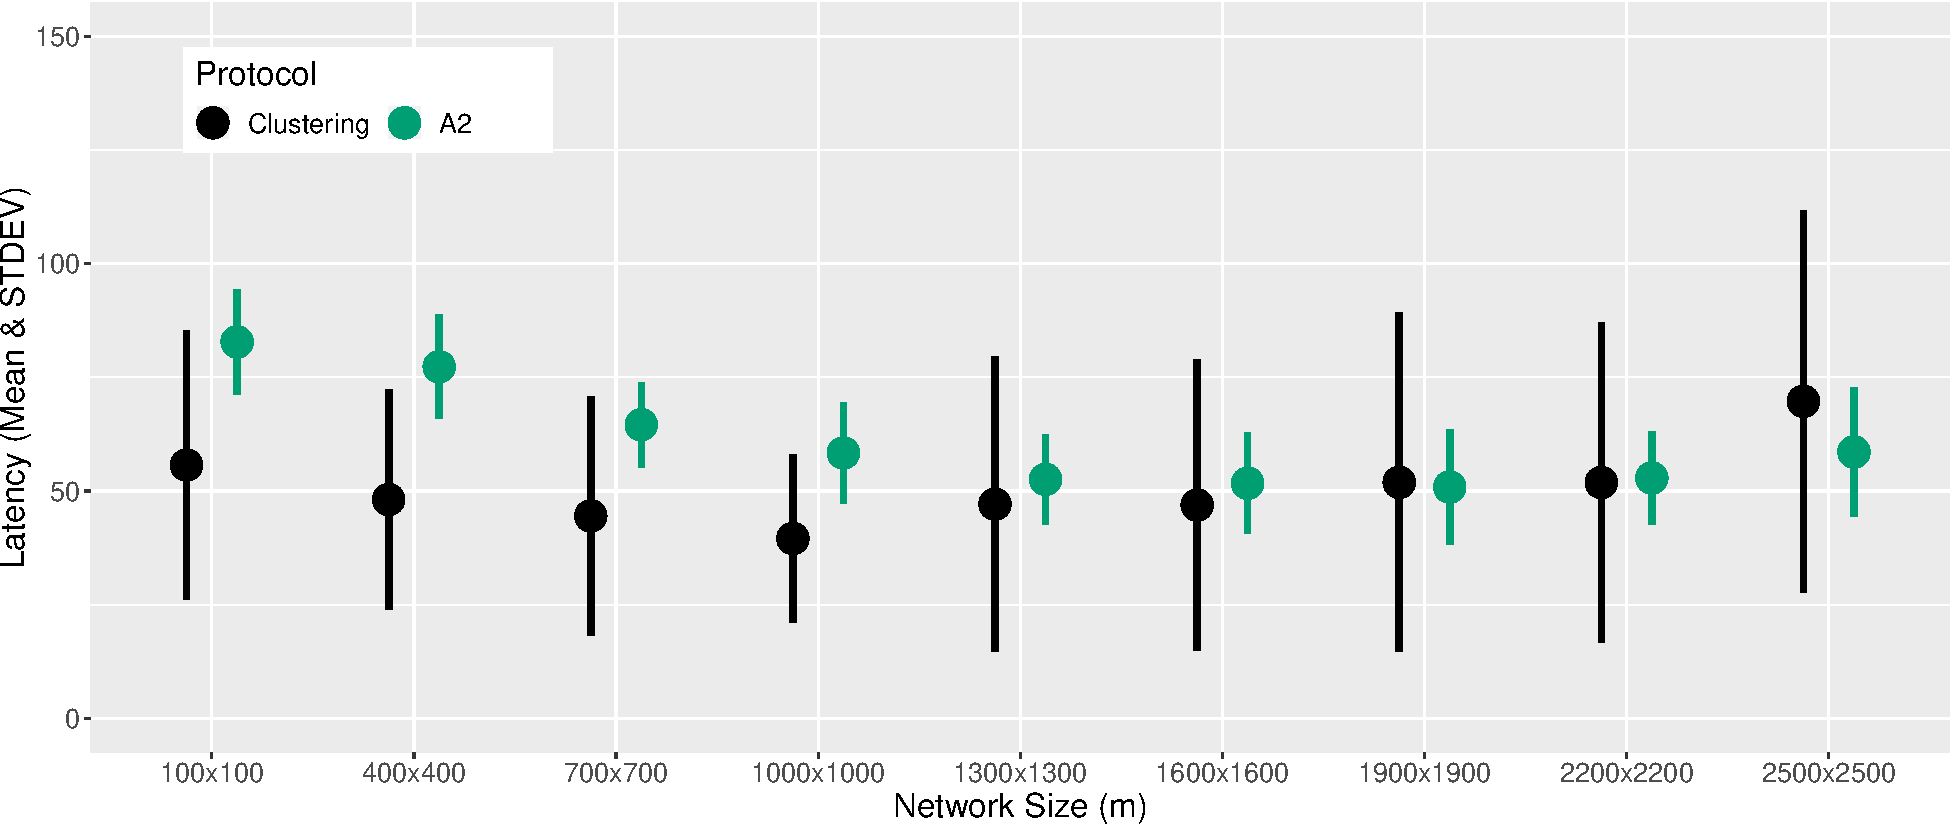
\includegraphics[width=\textwidth]{figure/Results/ChaosComparison/ChaosComparison_50_Latency.pdf}
        \caption{Networks with 50 nodes.}
        \label{subfig:latency-50-nodes}
    \end{subfigure}
    \hfill
    \begin{subfigure}{0.7\textwidth}
        \centering
        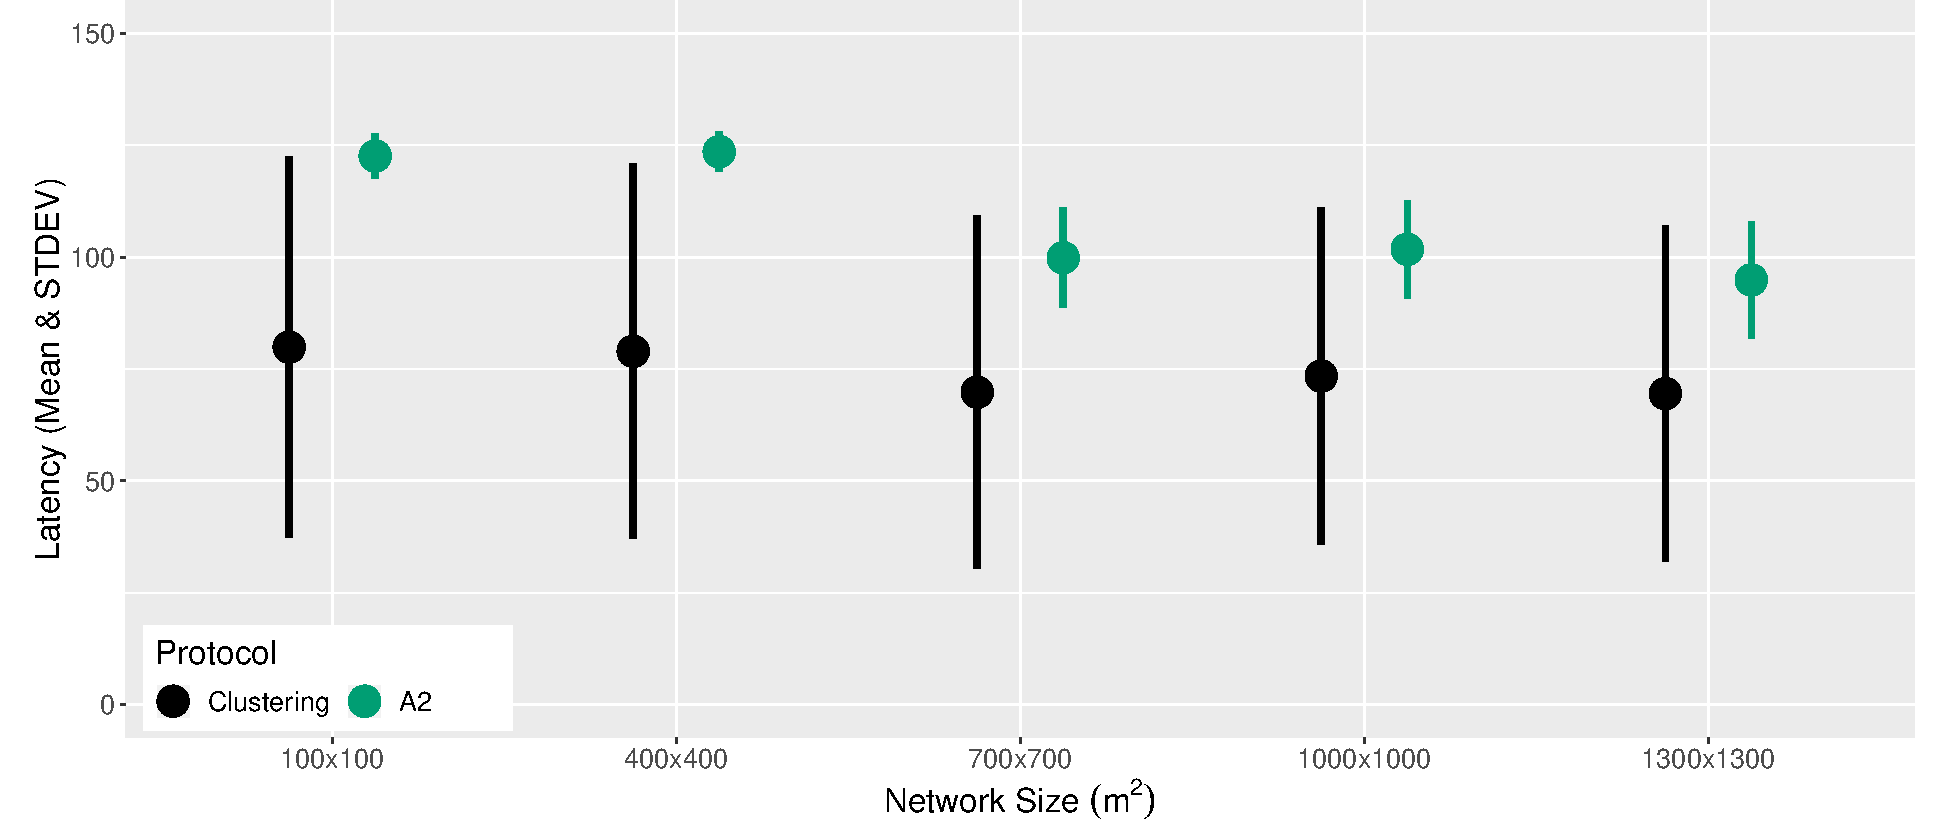
\includegraphics[width=\textwidth]{figure/Results/ChaosComparison/ChaosComparison_200_Latency.pdf}
        \caption{Networks with 200 nodes.}
        \label{subfig:latency-200-nodes}
    \end{subfigure}
    \caption{Latency comparison between \atwo{} with clustering and original \atwo{}.}
    \label{fig:latency-results}
\end{figure}

\subsection{Latency}
We show the mean latency and standard deviation for each test we run in \cref{fig:latency-results}. Looking at the tests using 50 nodes (\cref{subfig:latency-50-nodes}) our latency is on average a little lower than \atwo{} but with a higher standard deviation. We see a similar trend for 200 nodes (\cref{subfig:latency-200-nodes}) where our clustering consistently has lower latency for all topologies tested. 

We expect to see a lower latency on average, especially for 200 nodes, since each cluster has to handle a smaller amount of nodes while \atwo{} without clustering always has to handle all 200 nodes in the network. However, we have to take into account that our solution has much lower reliability than \atwo{}. Since we only measure the latency when the max application is running, if some nodes spend much time either associating or running another application (such as the join service) we do not count the latency for those nodes. Thus, for tests with lower reliability, we will have fewer data points for the latency measurements than for tests with higher reliability.

Furthermore, we have to take into account that we split the application rounds into cluster and cluster head rounds, which means that we effectively require two rounds to complete an application, rather than one. Thus we could argue that the actual latency for our application is twice the number that we depict in the graph, which would make our solution considerably slower than \atwo{}.

\begin{figure}[bt]
    \centering
    \begin{subfigure}{0.7\textwidth}
        \centering
        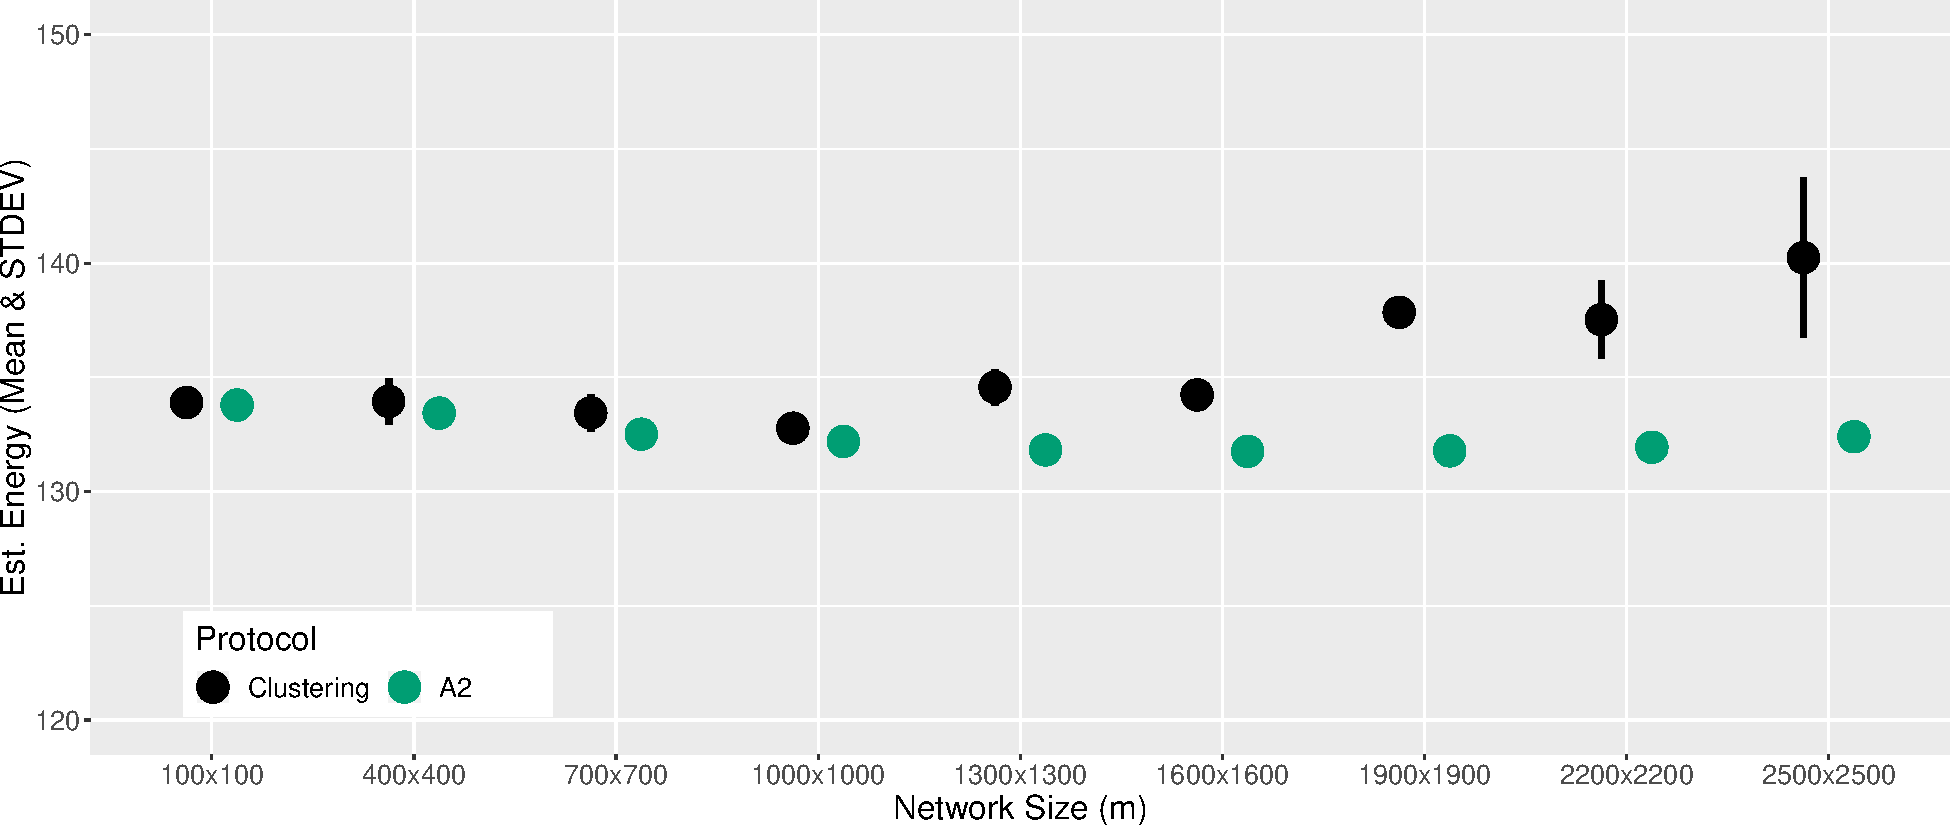
\includegraphics[width=\textwidth]{figure/Results/ChaosComparison/ChaosComparison_50_Energy.pdf}
        \caption{Networks with 50 nodes.}
        \label{subfig:energy-50-nodes}
    \end{subfigure}
    \hfill
    \begin{subfigure}{0.7\textwidth}
        \centering
        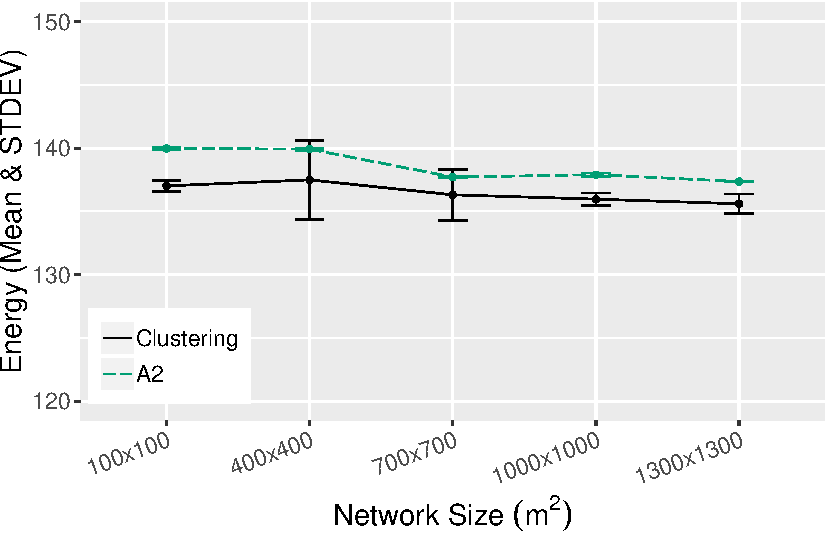
\includegraphics[width=\textwidth]{figure/Results/ChaosComparison/ChaosComparison_200_Energy.pdf}
        \caption{Networks with 200 nodes.}
        \label{subfig:energy-200-nodes}
    \end{subfigure}
    \caption{Energy comparison between \atwo{} with clustering and original \atwo{}.}
    \label{fig:energy-results}
\end{figure}


\subsection{Energy}
In \cref{fig:energy-results}, we plot the average energy usage per node per Energest time unit. The unit of the measurement is of less importance. What we look at here is the trend when increasing the area of the networks and how it shifts for the two different number of nodes. We observe in \cref{subfig:energy-50-nodes} that the energy usage for clustering increases with network area. The energy usage increases because the reliability drops, as we can see in \cref{subfig:reliability-50-nodes}; the decreasing reliability is due to nodes triggering resynchronisation meaning they enter the association phase which uses more energy since nodes do not sleep when they are trying to associate with the network.

Comparing 50 to 200 nodes we notice a higher energy usage on average for 200 nodes, this is expected for \atwo{} since more nodes imply more communication and longer rounds, which directly leads to higher energy consumption. Clustering shows a small advantage in the 200 network \cref{subfig:energy-200-nodes}, compared to the \atwo{} protocol; each cluster can reach consensus in fewer slots than the whole network can, and it is probably the reason why our average energy usage is slightly lower in all topologies. Besides these observations the trends in 50 and 200 nodes are similar.



\subsection{Flocklab}
We evaluate the \atwo{} protocol with and without clustering on the Flocklab testbed. We run both protocols four times for 30 minutes and calculate the mean and standard deviation of the latency, reliability, and estimated energy consumption; We can see the results from these tests in \cref{fig:flocklab-results}. It is clear that \atwo{} outperforms our solution in all metrics, achieving a significantly lower latency, higher reliability, and lower energy consumption.

There are probably several reasons for the difference in performance. First, our clustering solution is sometimes unstable, especially in smaller, sparser networks. In a small network and the presence of external interference, our solution does not perform well. Second, the Flocklab network is probably not a good candidate for clustering. As we have discussed previously, applying clustering to a network without taking into account its density and node count will produce poor results.

Additionally, we can look at the topology of Flocklab, which we show in \cref{fig:flocklab-topology}, to further explore our results. During the tests we run, the nodes located in the top left corner (1, 2, 4, 8, and 15) spend almost all of their time trying to associate with the network, unless the clustering service elects one of them as CH. When one of them is a CH, we get marginally better results since they have an easier time to get the correct max value. This show that, in some cases, our clustering can be heavily location dependent.

One thing to note is that the mean reliability for the \atwo{} protocol when we run our evaluation is approximately $86\%$. However, in the original evaluation of Chaos, Al Nahas et al.~achieved reliability of $99.9\%$ \cite{chaos-introduction-paper}. The large difference in reliability is mainly because we measure reliability differently. We have not collected the data needed to confirm their reliability results with the original reliability definition from Landsiedel et al.~\cite{chaos-introduction-paper}. However, the results presented from Cooja simulations in \cref{fig:reliability-result} does hold up to the results presented by Al Nahas et al.~\cite{a2-introduction-paper}, even under our stricter reliability definition.

\begin{figure}[bt]
    \centering
    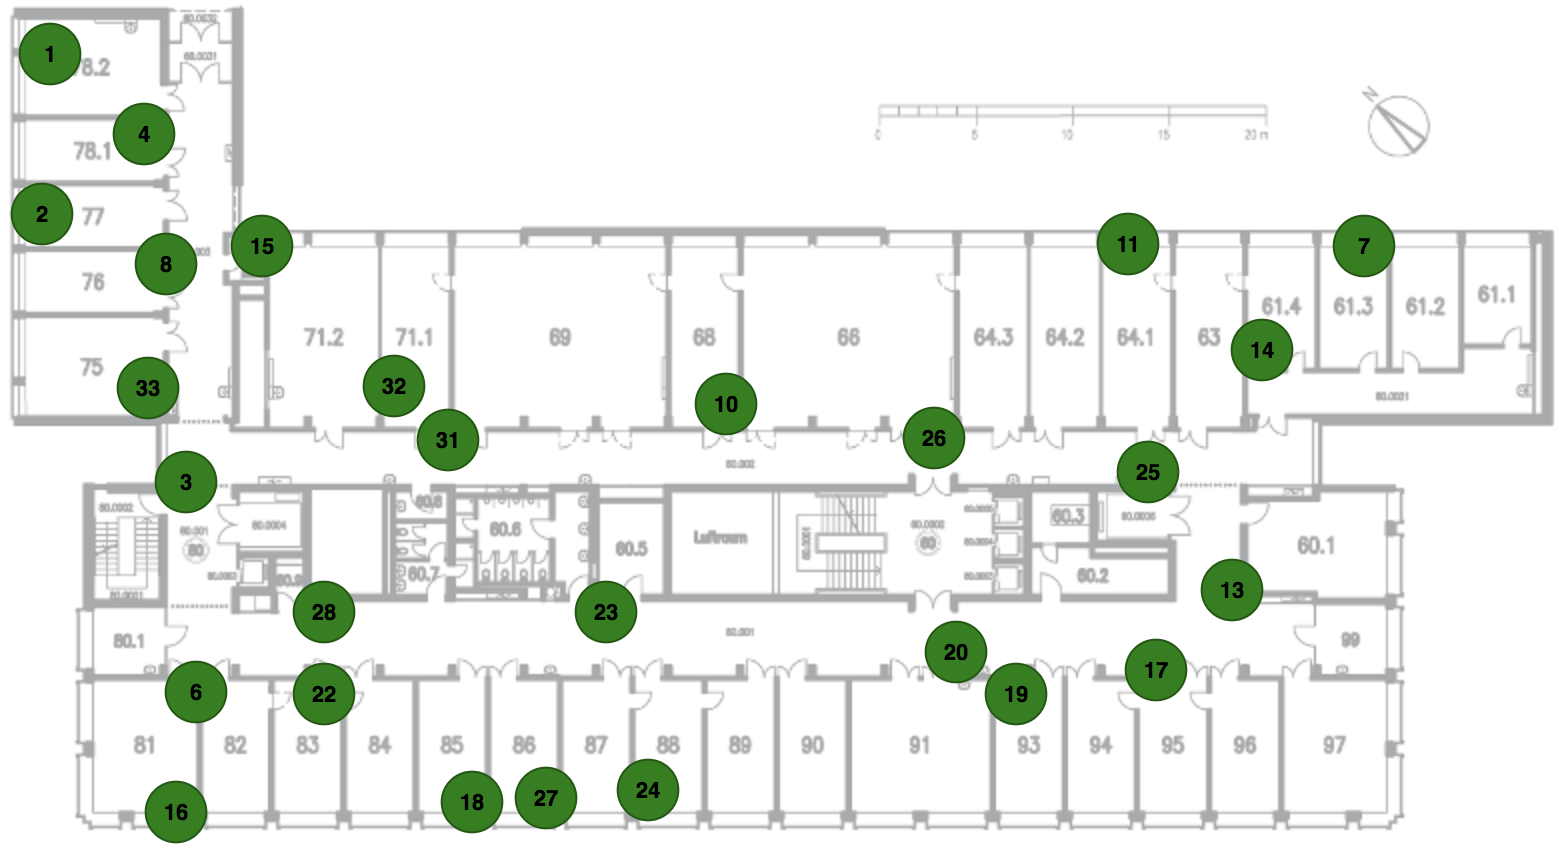
\includegraphics[width=0.75\textwidth]{figure/Results/ChaosComparison/Flocklab/FlocklabTopology.png}
    \caption{The topology of the Flocklab testbed \cite{Lim2013-flocklab-introduction}.}
    \label{fig:flocklab-topology}
\end{figure}

\begin{figure}[bt]
    \centering
        \begin{subfigure}{0.32\textwidth}
        \centering
        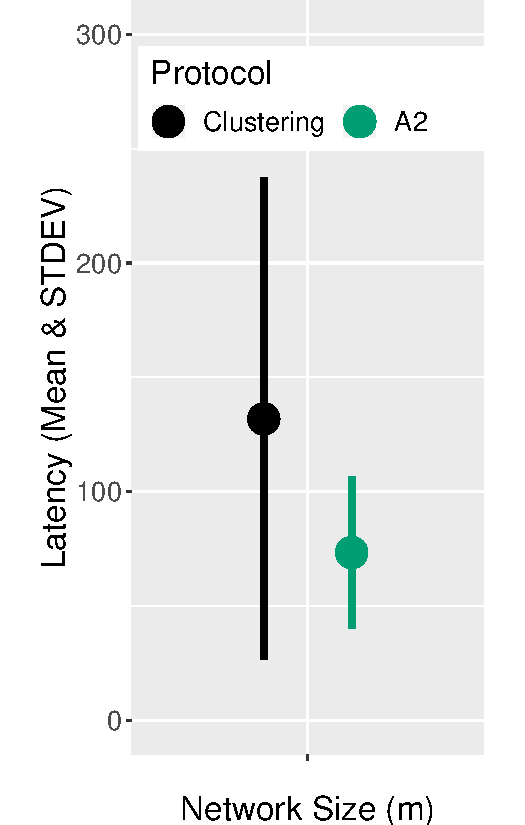
\includegraphics[width=\textwidth, keepaspectratio]{figure/Results/ChaosComparison/Flocklab/FlocklabComparison_Latency.pdf}
        \caption{Latency.}
        \label{subfig:flocklab-latency}
    \end{subfigure}
    \hfill
    \begin{subfigure}{0.32\textwidth}
        \centering
        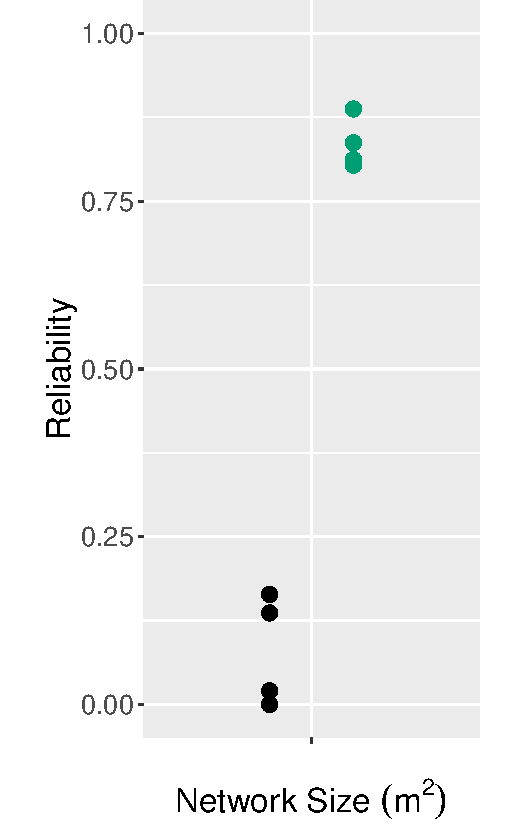
\includegraphics[width=\textwidth, keepaspectratio]{figure/Results/ChaosComparison/Flocklab/FlocklabComparison_Reliability.pdf}
        \caption{Reliability.}
        \label{subfig:flocklab-reliability}
    \end{subfigure}
    \begin{subfigure}{0.32\textwidth}
        \centering
        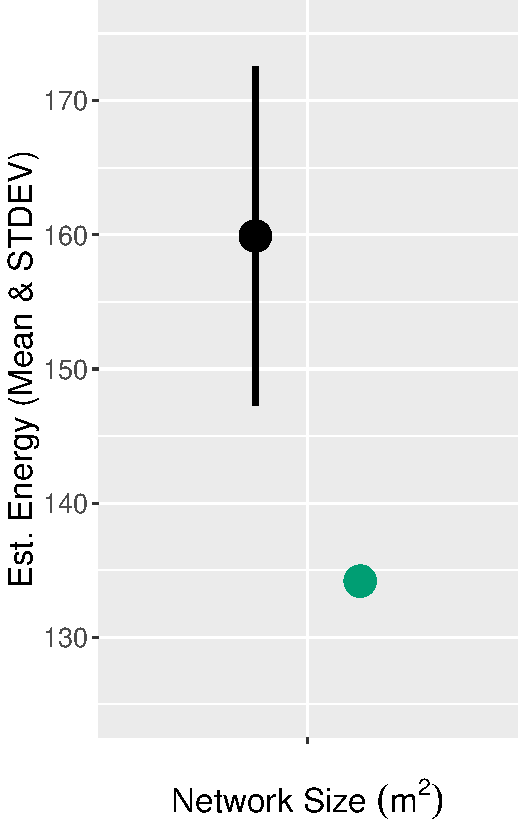
\includegraphics[width=\textwidth, keepaspectratio]{figure/Results/ChaosComparison/Flocklab/FlocklabComparison_Energy.pdf}
        \caption{Energy.}
        \label{subfig:flocklab-energy}
    \end{subfigure}
    \caption{The mean and standard deviation for the latency, reliability, and energy consumption for the Flocklab tests.}
    \label{fig:flocklab-results}
\end{figure}

\section{Discussion}
From our evaluation comparing \atwo{} and \atwo{} with clustering we conclude that using our clustering protocol performs at best as good as \atwo{} in every metric we measure. The most significant difference is in reliability, where we consistently have significantly lower reliability than \atwo{}. For the metrics latency and energy we are on par or even in the case of latency, a bit better, than \atwo{} we have to take into consideration that our clustering protocol performs only half as many application runs as \atwo{}, due to the interleaving cluster and CH rounds.

There are several possible reasons for these shortcomings, as we have mentioned previously, our clustering implementation is somewhat unstable. Because we switch which nodes considers themselves initiators, the network can end up in a state where no node consider themselves initiator. In a worst-case scenario, the tests will have $0\%$ reliability, because the network has never executed the application leaving us with no reliability data. This scenario may occur at any point during the execution, but we observe it happen more often at the times of reclustering when the dedicated initiator should return as coordinator, which is at round 200 and 400. In these cases, we use the rounds which did provide reliability data while the missing data count as failures.

However, there also exist test runs where our reliability is comparable to \atwo{}; notably we got up to $98.4\%$ reliability for some of the tests. This demonstrates that we can achieve good performance with our clustering protocol under the right circumstances. However, it is difficult to tell what exactly those circumstances are. What we can observe is that these good runs generally create two or three clusters, all of which are relatively similar in their sizes. However, some runs with the same properties provide results with low reliability. Thus, a more thorough examination of the communication within clusters is required since we cannot draw conclusions only from the number of CHs elected and the number of nodes in each cluster.

We illustrate the fact that networks with very similar clustering can have drastically different reliability in \cref{fig:comparing-good-and-bad-clustering}. The network to the left in the figure (\cref{subfig:bad-clustering}) achieved reliability of $51.2\%$ while the network to the right in the figure (\cref{subfig:good-clustering}) achieved reliability of $98.6\%$. If we look at the heat map over which application is running in the networks at different times in \cref{fig:application-map-comparing-good-and-bad-clustering} we observe that in one of the networks the join application is scheduled periodically throughout the entire run, but not in the other network. Note that we compare rounds 1-199 in one network and rounds 200-399 in the other network, but this does not affect the comparison.

To understand why the bad test intermittently schedules the join application we have to look at the differences in the clusters in \cref{fig:comparing-good-and-bad-clustering}. Both networks are overall similarly clustered, the clusters are approximately the same size and located in the same places. However, two nodes have changed clusters, node 23 and node 40. When we looked at the raw data for this particular test run, we saw that it was primarily node 23 that had trouble joining its cluster, probably because it was too far away to get enough packets from its cluster. Therefore, it never could complete the join protocol. In contrast, in the good network, this does not happen, even though the two tests have created similar clusters.

\begin{figure}[bt]
    \centering
        \begin{subfigure}{0.49\textwidth}
        \centering
        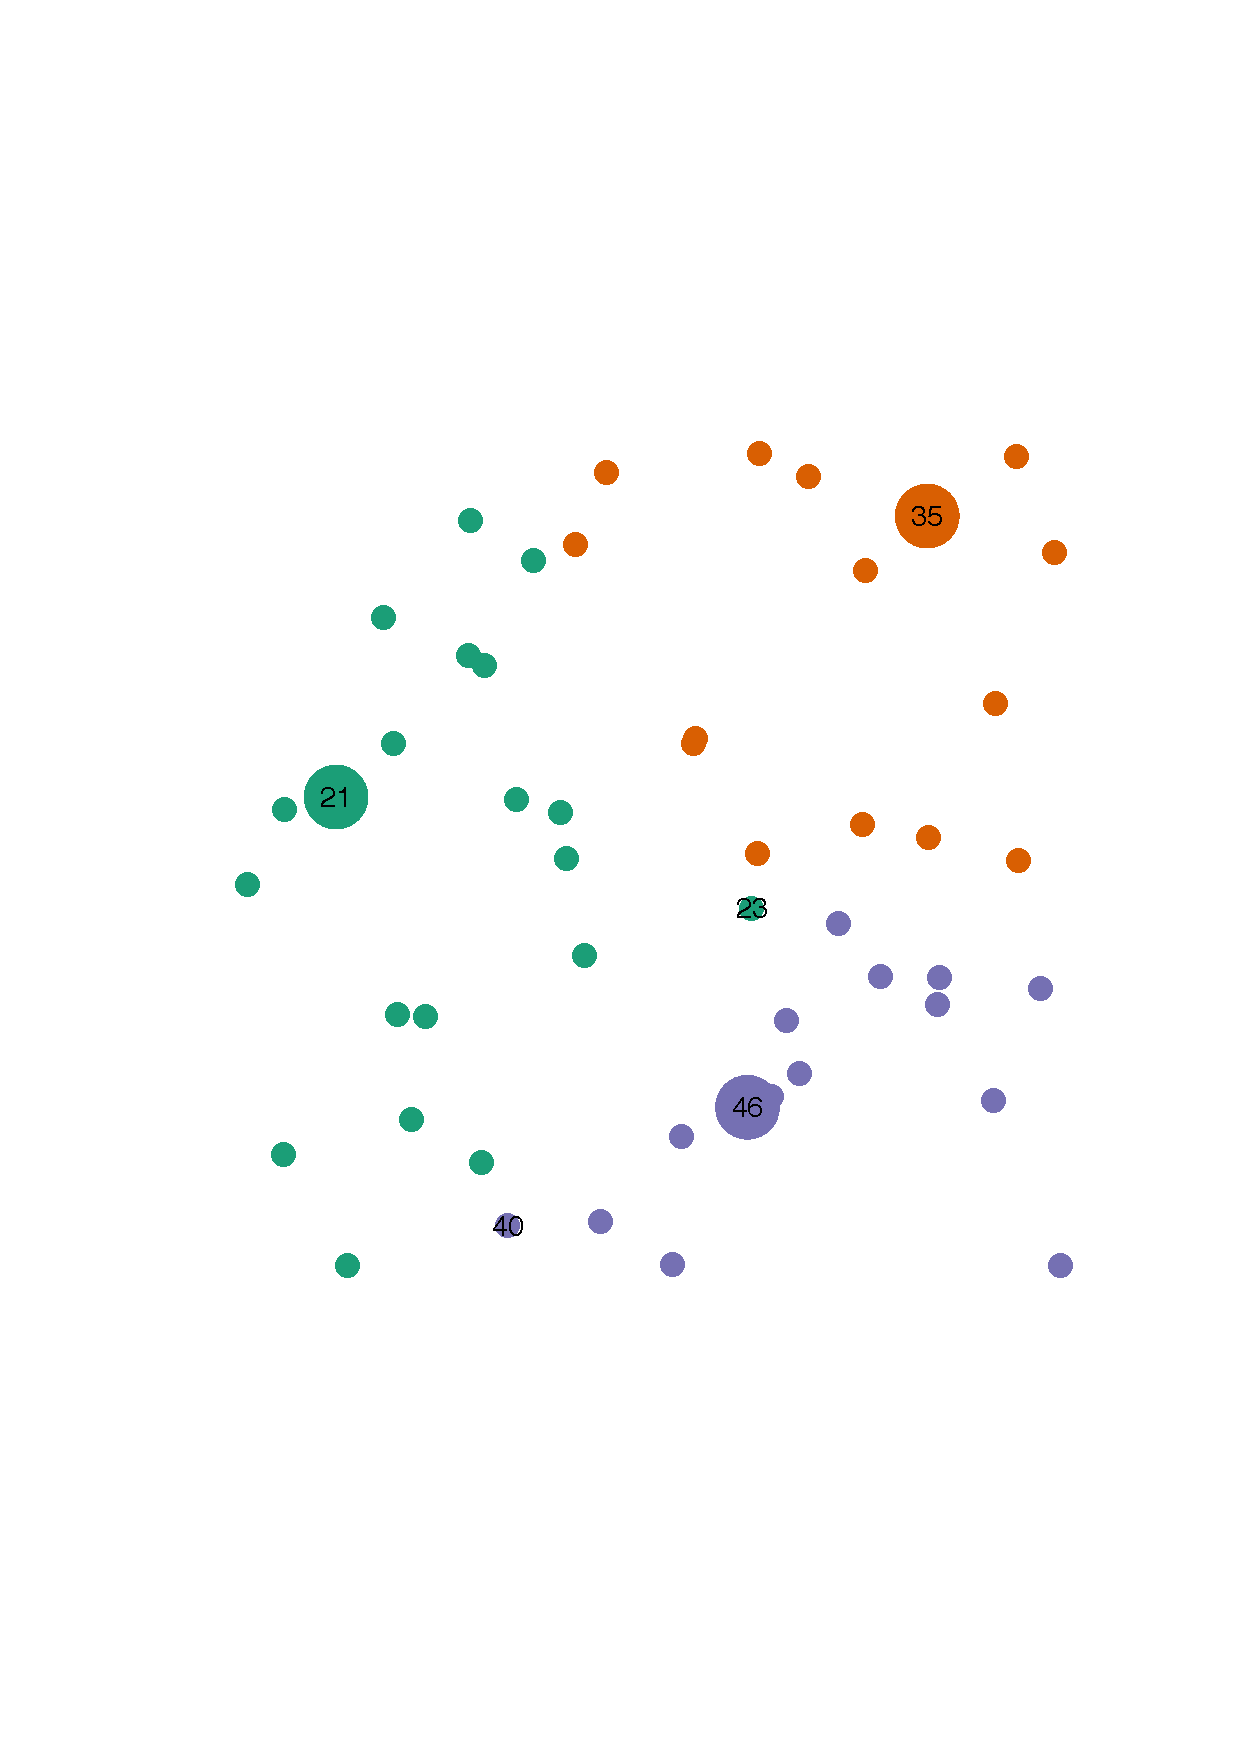
\includegraphics[width=\textwidth, keepaspectratio]{figure/Results/Discussion/ClusteringExample50nodes1000x1000maxOffRun1Bad.pdf}
        \caption{Clustering 50 nodes, achieving a reliability of $51.2\%$.}
        \label{subfig:bad-clustering}
    \end{subfigure}
    \hfill
    \begin{subfigure}{0.49\textwidth}
        \centering
        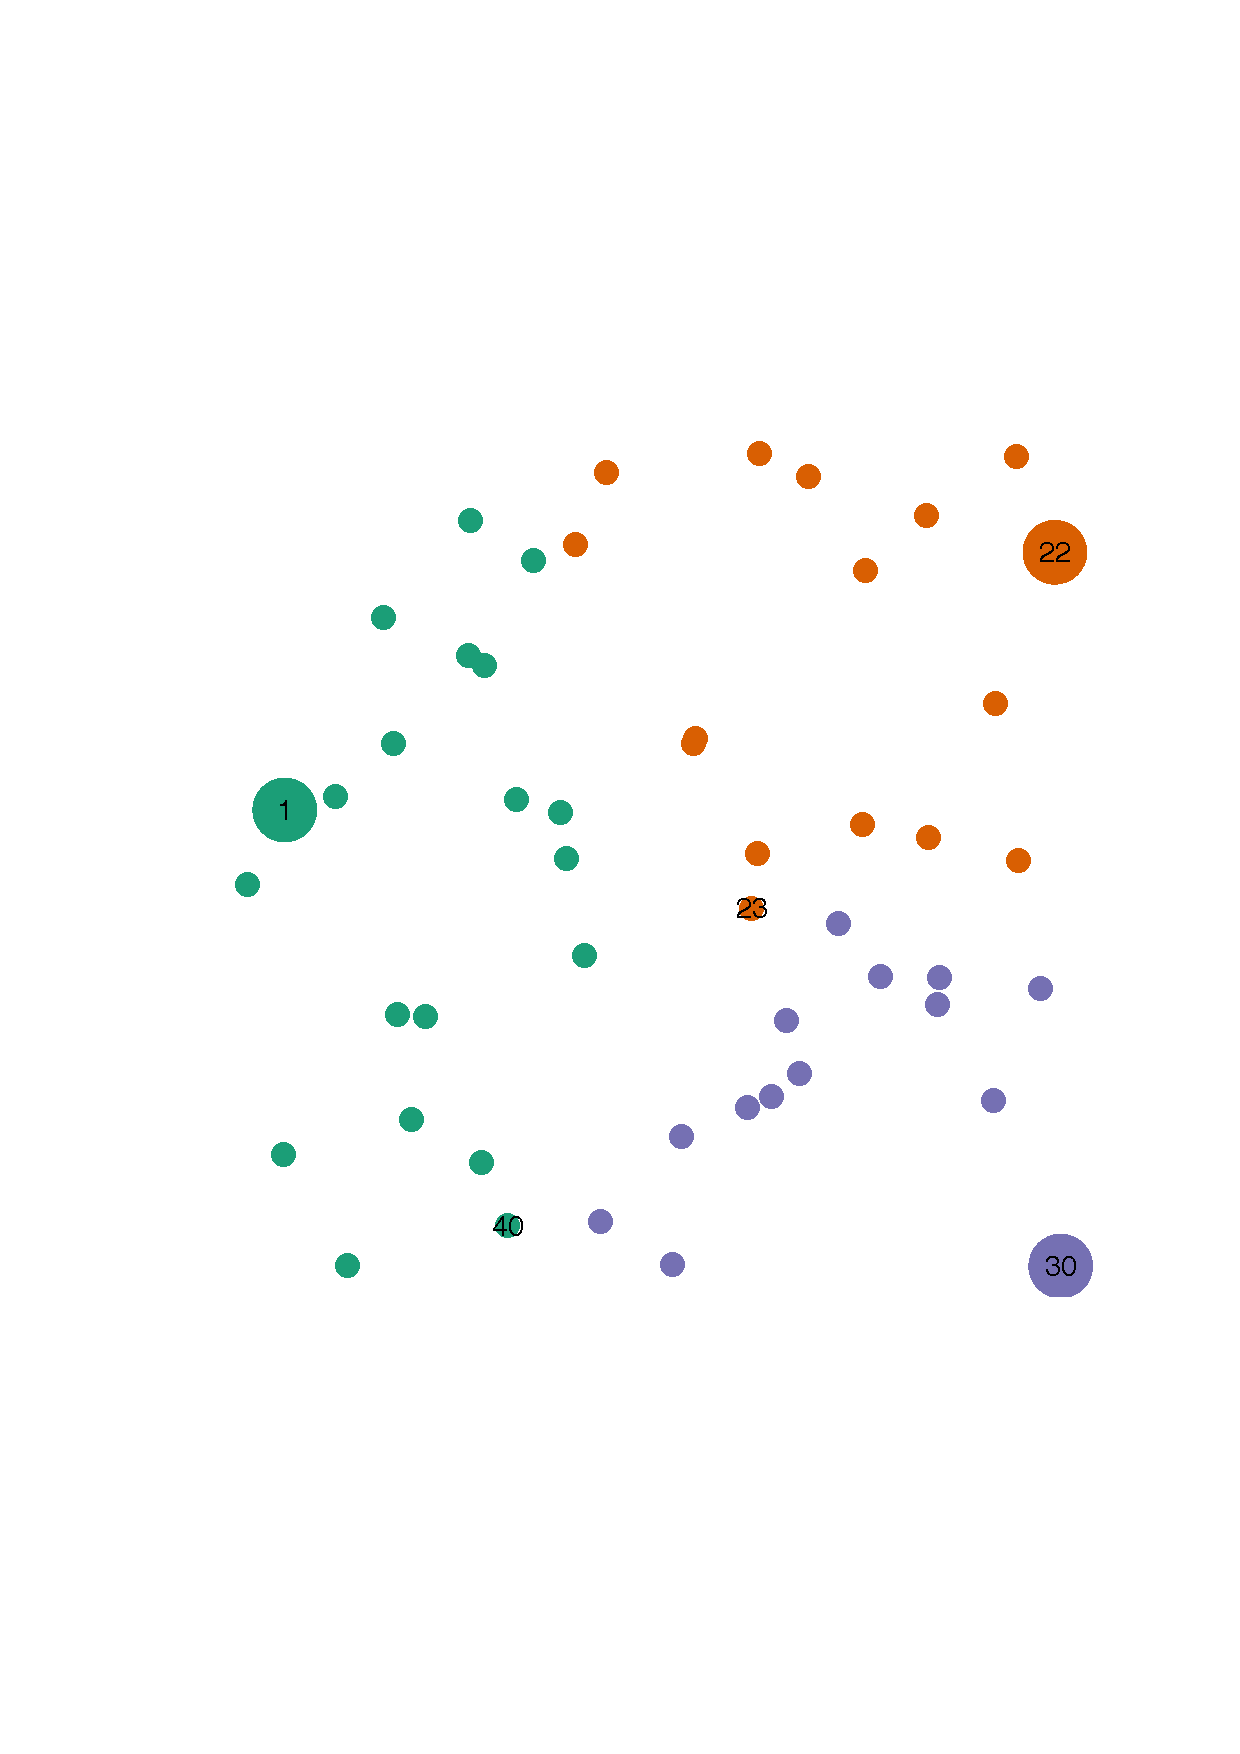
\includegraphics[width=\textwidth, keepaspectratio]{figure/Results/Discussion/ClusteringExample50nodes1000x1000maxOffRun5Good.pdf}
        \caption{Clustering 50 nodes, achieving a reliability of $98.6\%$.}
        \label{subfig:good-clustering}
    \end{subfigure}
    \caption{An example of two networks with an area of 1000x1000 and very similar clustering but with a significant difference in reliability.}
    \label{fig:comparing-good-and-bad-clustering}
\end{figure}

\subsection{Calculating the Reliability of a Network}
The way we chose to calculate the reliability of a network may have been unnecessarily strict. Here, we give three scenarios where our reliability calculation might be too strict.

First, in \cref{subsec:evaluation-reliability} we look at \cref{fig:reliability-result} and observe that the reliability of the clustered network topology in an area of 100x100 with 50 nodes is a lot higher than for 200 nodes. The reason for this significant difference in reliability is due to that the network with 200 nodes schedules the join service intermittently during the execution of the test, as can be seen in \cref{fig:application-map-50-nodes} and \cref{fig:application-map-200-nodes}. The pink dots represent the join service, and the yellow dots represent the max application. However, scheduling the join service should be an expected operation for a network to provide basic fault tolerance. 

Second, because we schedule CH rounds statically every other round, the network could run the first instance of the max application during a CH round; it depends on how many join rounds the network required after the demote phase. If max is run first in a CH round, and the node with the highest ID is not a CH, then this round will automatically fail. We do not take this into account when calculating the reliability of a test run since it should happen infrequently.

Third, the way we calculate reliability can be argued to have an unavoidably decreasing trend when the amount of nodes in the network increases. If a single node fails, the whole round counts as a fail for all clusters, even if some are successful. Hence, more nodes lead to a higher probability of a single failure, which means a higher probability for a failed round.

\begin{figure}[bt]
    \centering
        \begin{subfigure}{\textwidth}
        \centering
        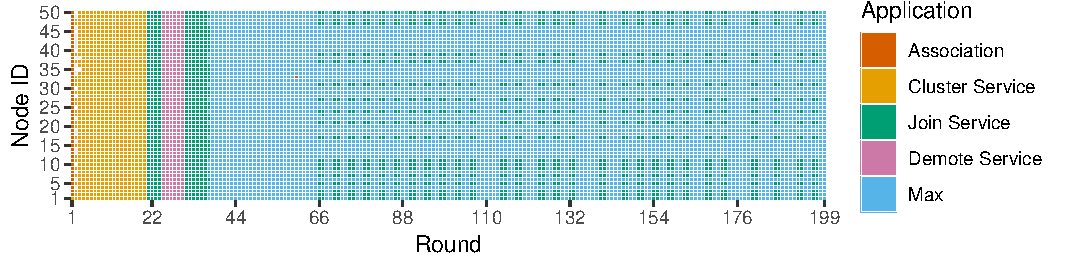
\includegraphics[width=\textwidth, keepaspectratio]{figure/Results/Discussion/applicationmap-50nodes-1000x1000-max-off-run1-bad.pdf}
        \caption{Some nodes are unable to join and therefore frequently schedule the join service resulting in a reliability of $51.2\%$.}
        \label{subfig:application-map-bad-clustering}
    \end{subfigure}
    \hfill
    \begin{subfigure}{\textwidth}
        \centering
        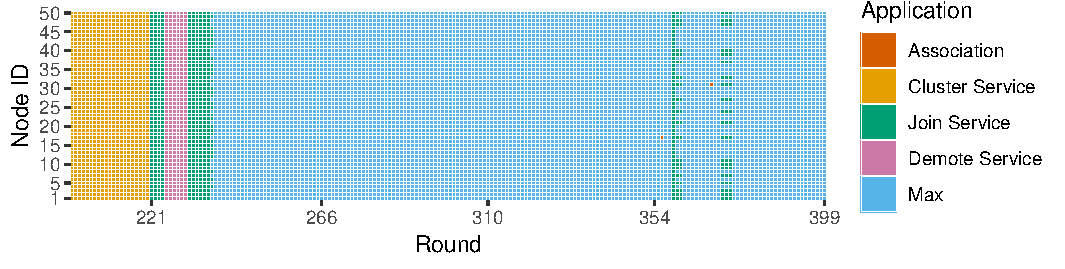
\includegraphics[width=\textwidth, keepaspectratio]{figure/Results/Discussion/applicationmap-50nodes-1000x1000-max-off-run5-good.pdf}
        \caption{A good run with few interruptions due to nodes scheduling the join service resulting in a reliability of $98.6\%$.}
        \label{subfig:application-map-good-clustering}
    \end{subfigure}
    \caption{An example of two application maps for two networks with 50 nodes and an area of 1000x1000 meters.}
    \label{fig:application-map-comparing-good-and-bad-clustering}
\end{figure}

\begin{figure}[H]
    \centering
    \begin{subfigure}{\textwidth}
        \centering
        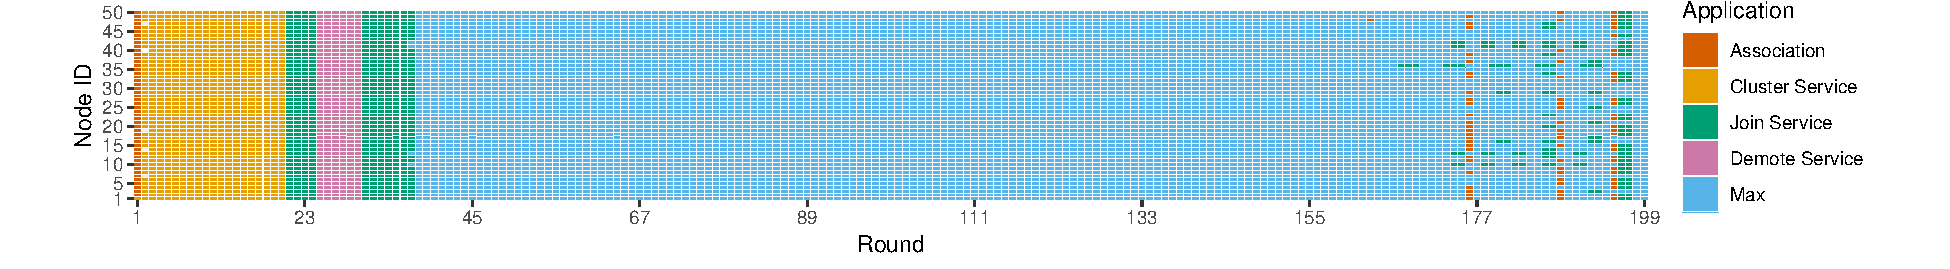
\includegraphics[width=\textwidth]{figure/Results/ReliabilityDiscussionApplicationHeatmaps/applicationmap50x50_1.pdf}
        \label{subfig:application-map-50-nodes-round-1-199}
    \end{subfigure}
    \hfill
    \begin{subfigure}{\textwidth}
        \centering
        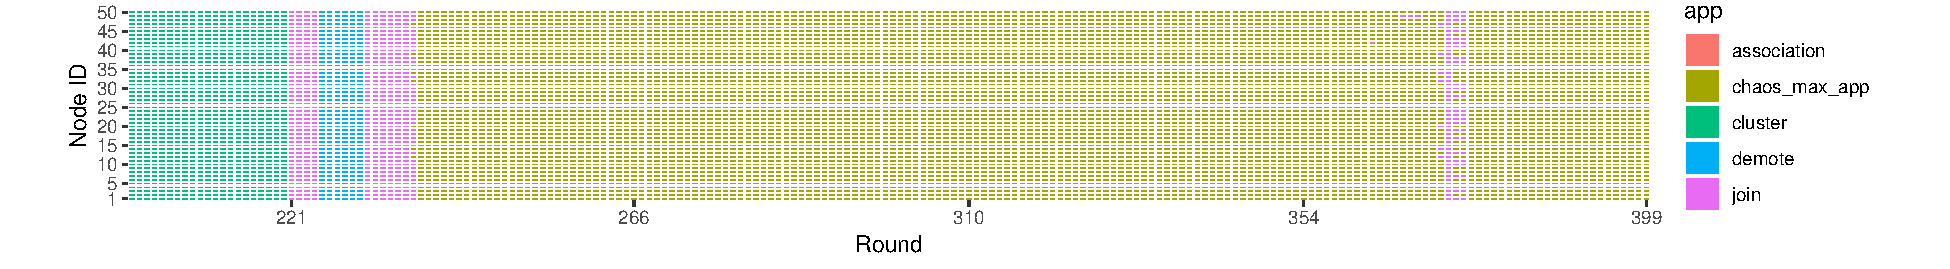
\includegraphics[width=\textwidth]{figure/Results/ReliabilityDiscussionApplicationHeatmaps/applicationmap50x50_2.pdf}
        \label{subfig:application-map-50-nodes-round-200-399}
    \end{subfigure}
    \begin{subfigure}{\textwidth}
        \centering
        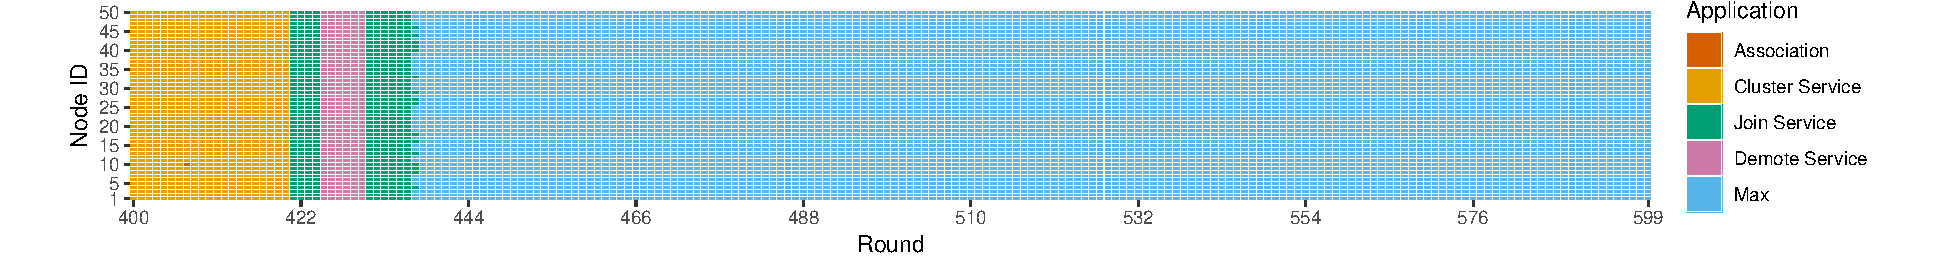
\includegraphics[width=\textwidth]{figure/Results/ReliabilityDiscussionApplicationHeatmaps/applicationmap50x50_3.pdf}
        \label{subfig:application-map-50-nodes-round-400-599}
    \end{subfigure}
    \caption{Application heat map of a test with 50 nodes over a 100x100 network area executing 600 rounds. Join is rarely executed outside its specified schedule.}
    \label{fig:application-map-50-nodes}
\end{figure}
\begin{figure}[H]
\label{fig:application-map-200-nodes}
    \centering
    \begin{subfigure}{0.9\textwidth}
        \centering
        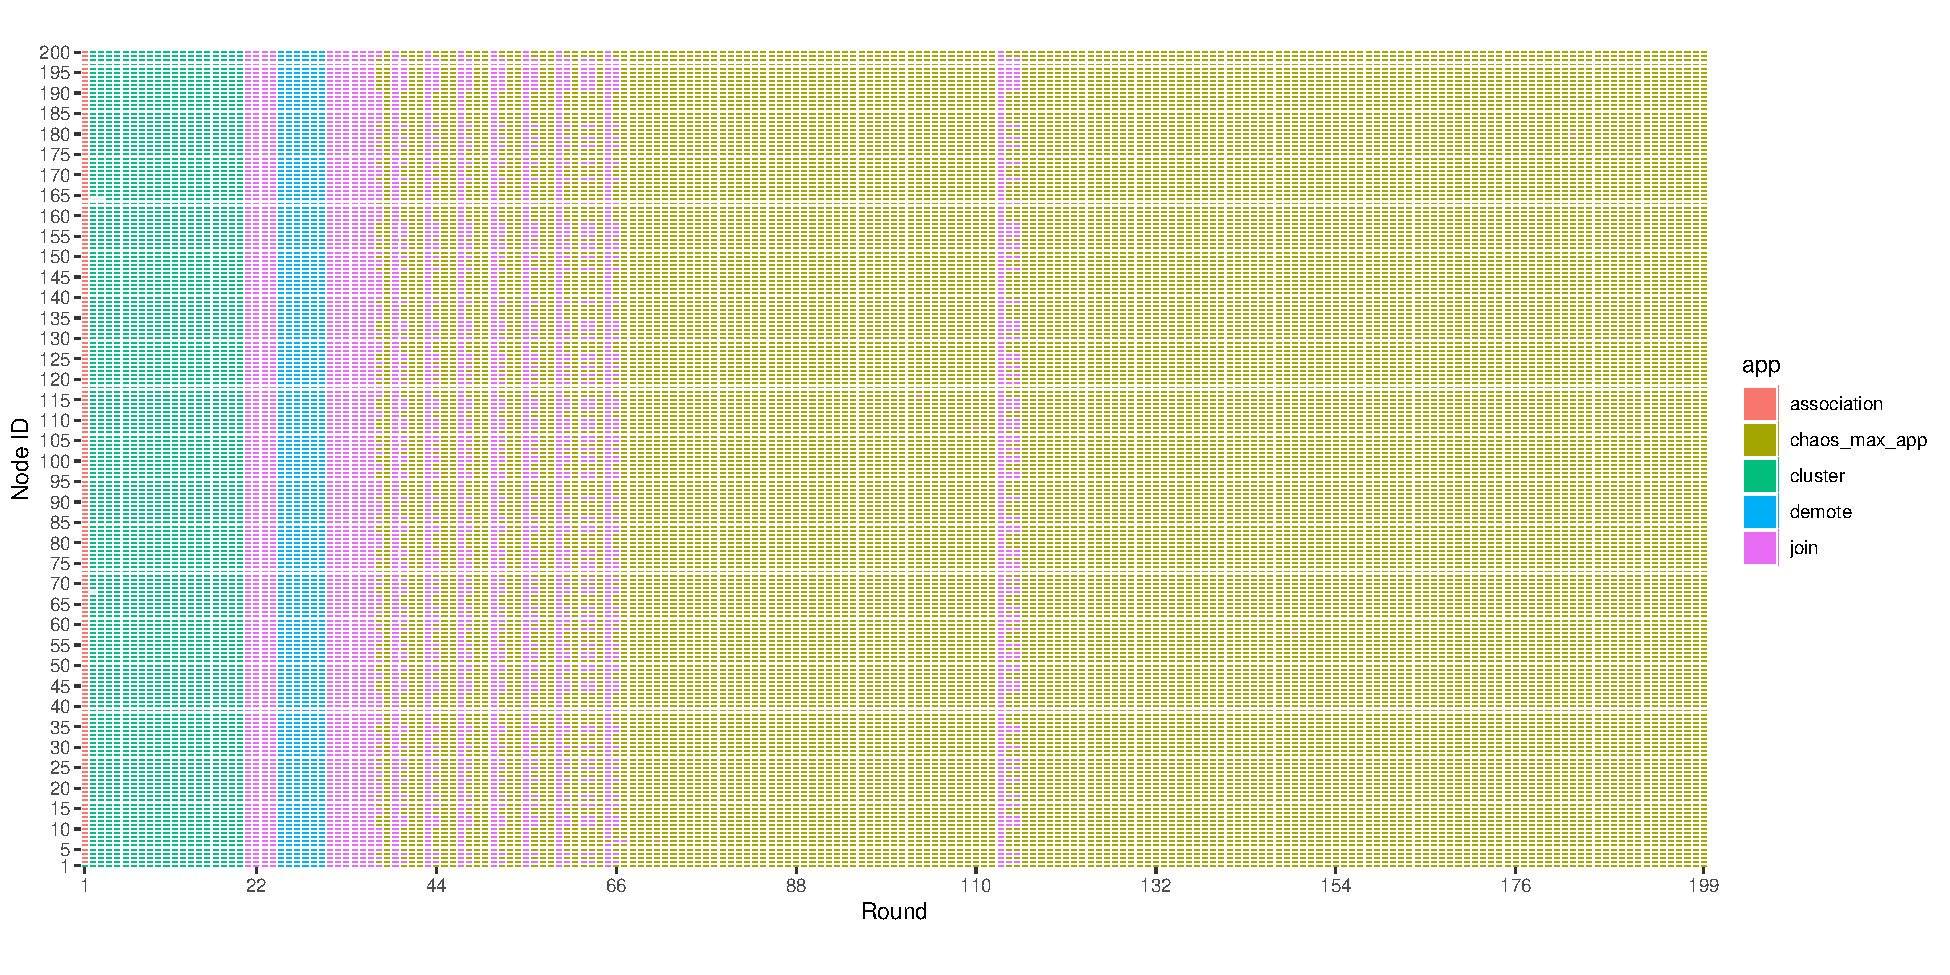
\includegraphics[width=\textwidth]{figure/Results/ReliabilityDiscussionApplicationHeatmaps/applicationmap200x200_1.pdf}
        \label{subfig:application-map-200-nodes-round-1-199}
    \end{subfigure}
    \hfill
    \begin{subfigure}{0.9\textwidth}
        \centering
        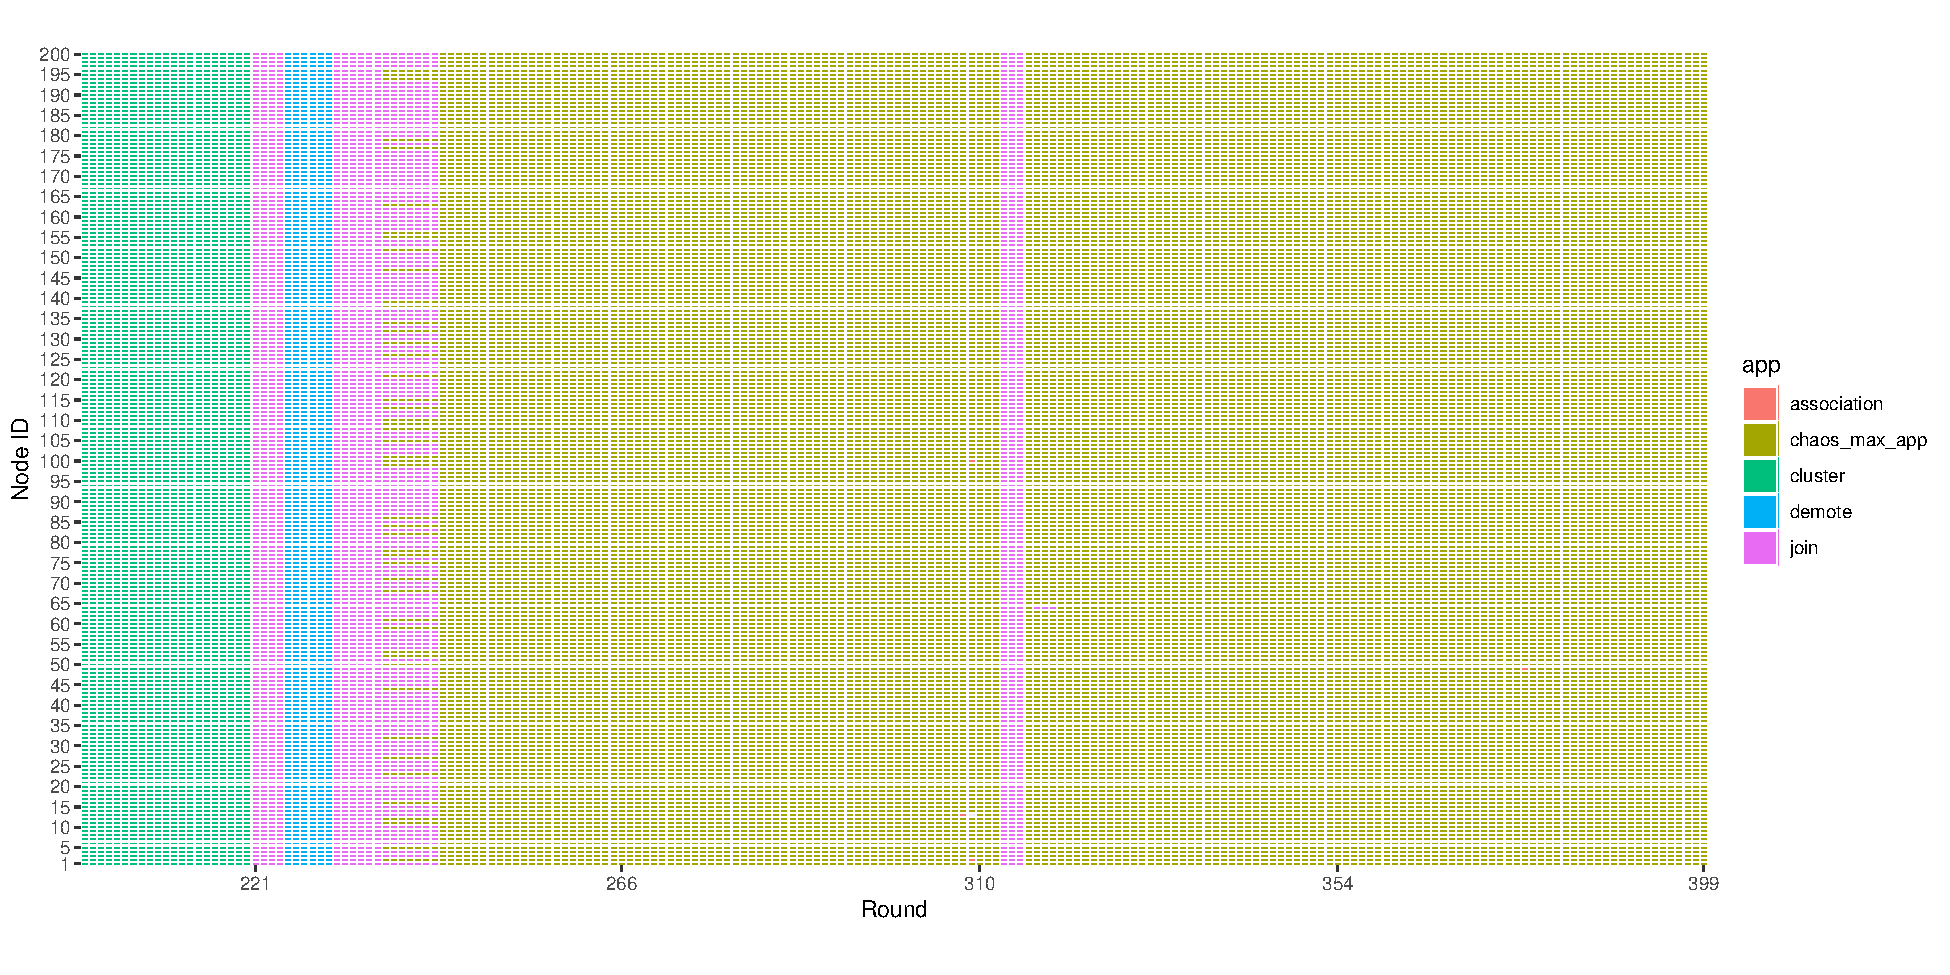
\includegraphics[width=\textwidth]{figure/Results/ReliabilityDiscussionApplicationHeatmaps/applicationmap200x200_2.pdf}
        \label{subfig:application-map-200-nodes-round-200-399}
    \end{subfigure}
    \begin{subfigure}{0.9\textwidth}
        \centering
        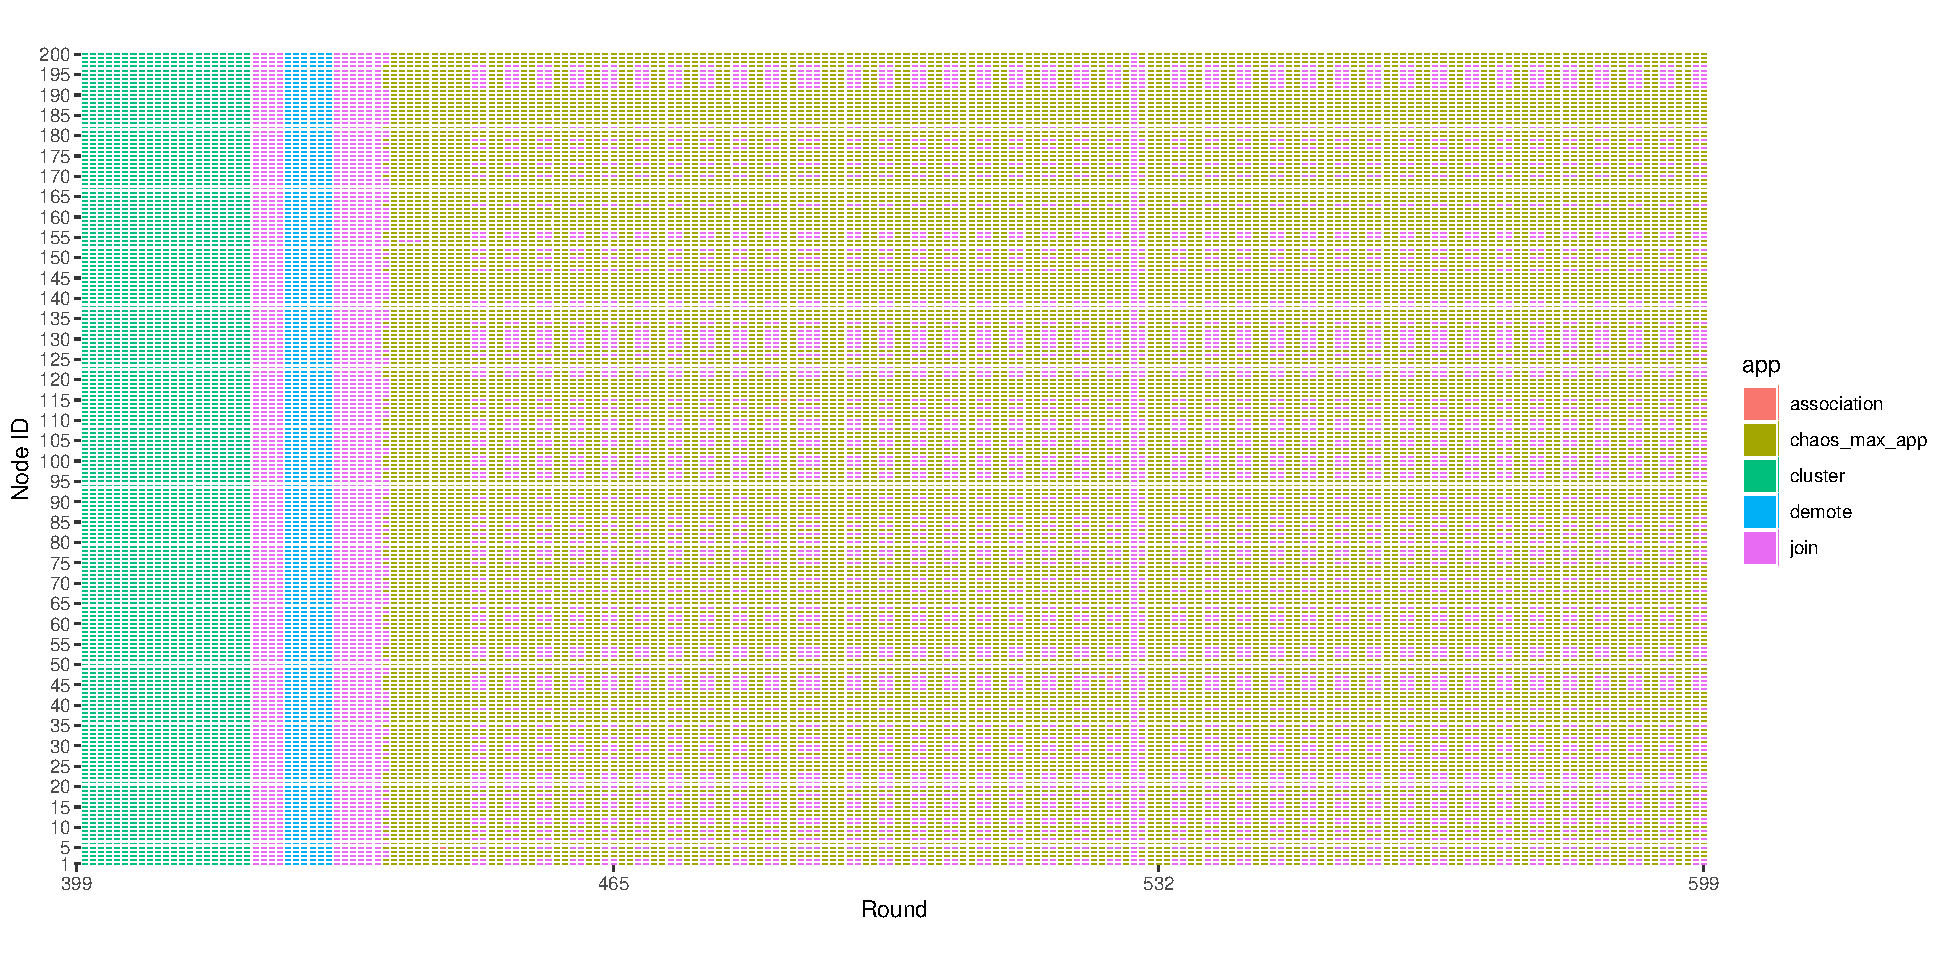
\includegraphics[width=\textwidth]{figure/Results/ReliabilityDiscussionApplicationHeatmaps/applicationmap200x200__3.pdf}
        \label{subfig:application-map-200-nodes-round-400-599}
    \end{subfigure}
    \caption{Application heat map of a test with 200 nodes over a 100x100 network area executing 600 rounds. Some clusters often execute join, especially after the last clustering occurring in rounds 400 to 437}
\end{figure}

